\documentclass[11pt,a4paper]{report}

% Aberstwyth dissertation LaTeX Template
% Authors: Dr. Hannah Dee (hmd1@aber.ac.uk), Neil Taylor (nst@aber.ac.uk)
% This has been adapted from the Leeds Thesis template and the 
% Group Project template for Computer Science in Aberystywth University.
% 
% All comments and suggestions welcome.
%
% Template designed to be used with pdflatex: it may need alteration to
% run with a different LaTeX engine.
%
% Note - this is offered as a starting point for your work. You are not 
% required to use this template and can choose to create your own document 
% without it. 

% To build document on the unix command line, run four commands:
 
% pdflatex dissertation
% bibtex dissertation
% pdflatex dissertation
% pdflatex dissertation

% you will end up with dissertation.pdf 
\usepackage{mmp}
\usepackage{pdfpages}
\usepackage{todonotes}
\usepackage{hyperref}
\usepackage{csquotes}
\usepackage{minted}
\usepackage[nodayofweek,level]{datetime}

% this is the recomneded font encoding so that you can use non aski chariters
\usepackage[T1]{fontenc}

\definecolor{red}{RGB}{240,26,36}
\definecolor{green}{RGB}{22,157,91}

\usepackage{tikz}
\usetikzlibrary{shapes.geometric, arrows}
\tikzstyle{startstop} = [rectangle, rounded corners, minimum width=3cm, minimum height=1cm,text width=3cm, text centered, draw=black, fill=red!70]
\tikzstyle{process} = [rectangle, minimum width=3cm, minimum height=1cm, text centered, text width=3cm, draw=black, fill=orange!70]
\tikzstyle{decision} = [diamond, minimum width=3cm, minimum height=1cm, text centered, text width=3cm, draw=black, fill=green!70]

\tikzstyle{arrow} = [draw, -latex']
% \tikzstyle{arrow} = [thick,->,>=stealth]

% the following packages are used for citations - You only need to include one. 
%
% Use the cite package if you are using the numeric style (e.g. IEEEannot). 
% Use the natbib package if you are using the author-date style (e.g. authordate2annot). 
% Only use one of these and comment out the other one. 
\usepackage{cite}
%\usepackage{natbib}

\usepackage[toc]{glossaries}
\makeglossaries

% Use the following to selectively exclude chapters
%\includeonly{cover,abstract,acknowledge,declare,chapter1,chapter2}

\begin{document}

% all of the include directives below refer to tex files
% so 
\title{Computer control of the amateur radio ``Yaesu FT8900''}

% Your name
\author{Cormac Brady}

% Your email 
\authoremail{cob16@aber.ac.uk, cormacbrady@hotmail.co.uk}

\degreeschemecode{G401} %e.g. G400 
\degreeschemetitle{Computer Science} % e.g. Computer Science
\degreetype{BSc}

\modulecode{CS39440} % i.e. CS39440, CC39440, CS39620
\moduletitle{Major Project} % i.e. Major Project or Minor Project

\date{\today} % i.e. the date of this version of the report

\status{Release} % Use draft until you create the release version. Then, change this to Release.
\version{1.0}

%The title and name of your supervisor.
\supervisor{Dave Price BSc, MSc (Wales), MBCS} 

%The email for your supervisor. 
\supervisoremail{dap@aber.ac.uk}

\maketitle



 includes cover.tex - to change the content,
% edit the tex file

\pagenumbering{roman}

% This is the front page

\title{Computer control of the amateur radio ``Yaesu FT8900''}

% Your name
\author{Cormac Brady}

% Your email 
\authoremail{cob16@aber.ac.uk, cormacbrady@hotmail.co.uk}

\degreeschemecode{G401} %e.g. G400 
\degreeschemetitle{Computer Science} % e.g. Computer Science
\degreetype{BSc}

\modulecode{CS39440} % i.e. CS39440, CC39440, CS39620
\moduletitle{Major Project} % i.e. Major Project or Minor Project

\date{\today} % i.e. the date of this version of the report

\status{Release} % Use draft until you create the release version. Then, change this to Release.
\version{1.0}

%The title and name of your supervisor.
\supervisor{Dave Price BSc, MSc (Wales), MBCS} 

%The email for your supervisor. 
\supervisoremail{dap@aber.ac.uk}

\maketitle



 

% Set up page numbering
\pagestyle{empty}

% declarations of originality 
\thispagestyle{empty}

%%%
%%% You must sign the declaration of originality. 
%%%
%%% You are submitting this electronically. Therefore, to sign, you 
%%% type your name and date to replace the .... characters. 
%%%
\begin{center}
    {\LARGE\bf Declaration of originality}
\end{center}

I confirm that:

\begin{itemize}
\item{This submission is my own work, except where 
clearly indicated.}

\item{I understand that there are severe penalties for Unacceptable Academic Practice, which can lead to loss of marks or even the withholding of a degree.}
 
\item{I have read the regulations on Unacceptable Academic Practice from the University's Academic Quality and Records Office (AQRO) and the relevant sections of the current Student Handbook of the Department of Computer Science.}
 
\item{In submitting this work I understand and agree to abide by the University's regulations governing these issues.}
\end{itemize}

\vspace{2em}
\textbf{Name :} Cormac Brady  \\

\vspace{1em}
\textbf{Date :} \today\\

%%% 
%%% We would like to make a selection of final reports available to students that take 
%%% this module in future years. To enable us to do this, we require your consent. You 
%%% are not required that you do this, but if you do give your consent, then we will have 
%%% the option to select yours as one of a number of reports as examples for other 
%%% students. If you would like to give your consent, then please include the following 
%%% text and type your name and date to replace the .... characters. 
%%% 
%%% If you do not wish to give your consent, please remove this from your report. 
%%%
\vspace{1em}
\begin{center}
    {\LARGE\bf Consent to share this work}
\end{center}

By including my name below, I hereby agree to this dissertation being made available to other students and academic staff of the Aberystwyth Computer Science Department.  

\vspace{2em}
\textbf{Name :}  Cormac Brady  \\

\vspace{1em}
\textbf{Date :} \today \\


               

\thispagestyle{empty}

\begin{center}
    {\LARGE\bf Acknowledgements}
\end{center}

I would like to thank everyone for there support in helping me to produce this report. In particular, I would like to thank my support tutor, Heather Philips for helping me stay organised for the last three years of my degree. I would also like to thank my supervisor, Dave Price for his help in learning the details of amateur radio and its terminology. Many thanks also to Peter Todd, for his help with the physical side of the project as well as for putting up with my barrage of questions about serial and electronics. 

I would also like to thank my friends Owen Garland, Xander Barnes and Nicholas Dart for helping my studies at Aberystwyth University stay both focused and entertaining.

Of course I would never have even been able to even write this acknowledgement section without the enduring love and support of my parents, Mark and Christina. They helped me through my childhood and gave me the opportunity to find and pursue my interest in computing.

Finally I would like to thank Laura Pugh for all her love and support that she has given me throughout my undergraduate degree. She is the most kind person I know and has put up with me moving over 600km away to Germany for my industrial year.
 % Acknowledgements
\thispagestyle{empty}

\begin{center}
    {\LARGE\bf Abstract}
\end{center}

In amateur radio, C.A.T (Computer Aided Transceiving) is the name for a radio's ability to interact with a computer, often via serial communication. This is often done so that the radio can behave like a computer peripheral. There are many applications that rely on this premise to provide a user interface on a computer screen to fully control a radio.

The \gls{8900} is a popular budget amateur radio. However, the the \gls{8900} it is missing a significant feature, C.A.T (Computer Aided Transceiving). The design of the The \gls{8900} allows users the potential to add this feature to the radio. This is due to its ability to split off the front control surface from the main body. The detachment is made via a connecting serial line and is intended to be used to mount the controls of the radio in the console of a car. 

This report details the process of research, design and development of an application that is capable of controlling the radio, by tapping into this serial connection. The application was developed as an alternative to existing commercial solutions, with further consideration given to cost constraints. The typical conditions expected of CAT capable radios gave rise to strong efficiency and portability requirements. 

The end result was an application written in C that met it's objectives to produce a \gls{mvp}. The produced application has been evaluated for its quality and suitability as a solution.                 % Abstract

\pagenumbering{roman}
\pagestyle{fancy}
\fancyhead{}
\fancyfoot[C]{\thepage}
\renewcommand{\headrulewidth}{0 pt}
\renewcommand{\chaptermark}[1]{\markboth{#1}{}}

\tableofcontents   
\newpage
\listoffigures
\newpage 
\listoftables
\newpage

% Set up page numbering
\pagenumbering{arabic}

\setchapterheaderfooter

% include the chapters
\chapter{Background}

\begin{displayquote}
``Amateur radio is a popular technical hobby and volunteer public service that uses designated radio frequencies for non-commercial exchange of messages, wireless experimentation, self-training, and emergency communications.
Amateur Radio is the only hobby governed by international treaty.'' \cite{def_amateur_radio}
\end{displayquote}

Amateur radio operators do not always sit in front of their radios. Often for operators it is more convenient to control their radios remotely, known more commonly as having a ``remote shack''. In this scenario as much remote control as possible is desired. This is often achieved using existing commercial or home made solutions that rely on simply repeating control signals. For example the ``RRC 1258Mk'' is a product designed to do just. However it is priced at \$708\cite{RRC_1258Mk} making it often prohibitively expensive as it is two times the price of budget consumer radios. Instead it would be preferable to understand and/or emulate these signals. The end result is that the radio gains \gls{cat}\cite{CAT} features.

Remote shacks are geographically positioned for their prime transceiving properties, for example on the top of a hill so the signal is less affected by the geometry of the surrounding area. They are often limited in their connectivity to utilities, such as power or Internet connection. This is especially in extremely remote areas where communication is sometimes done over telephone networks. This adds some constraints to the project and is discussed in the next section.

An ideal scenario for these kind of users is where all functions can be controlled from the radio remotely, using as little data traffic as possible. This use-case also extends to users that prefer to use a PC to control their radios. This may be for more features, better user experience (given by software), or possibly for accessibility reasons (i.e where reading the screen or using the small dials would be a problem for the operator).

\begin{figure}
    \centering
    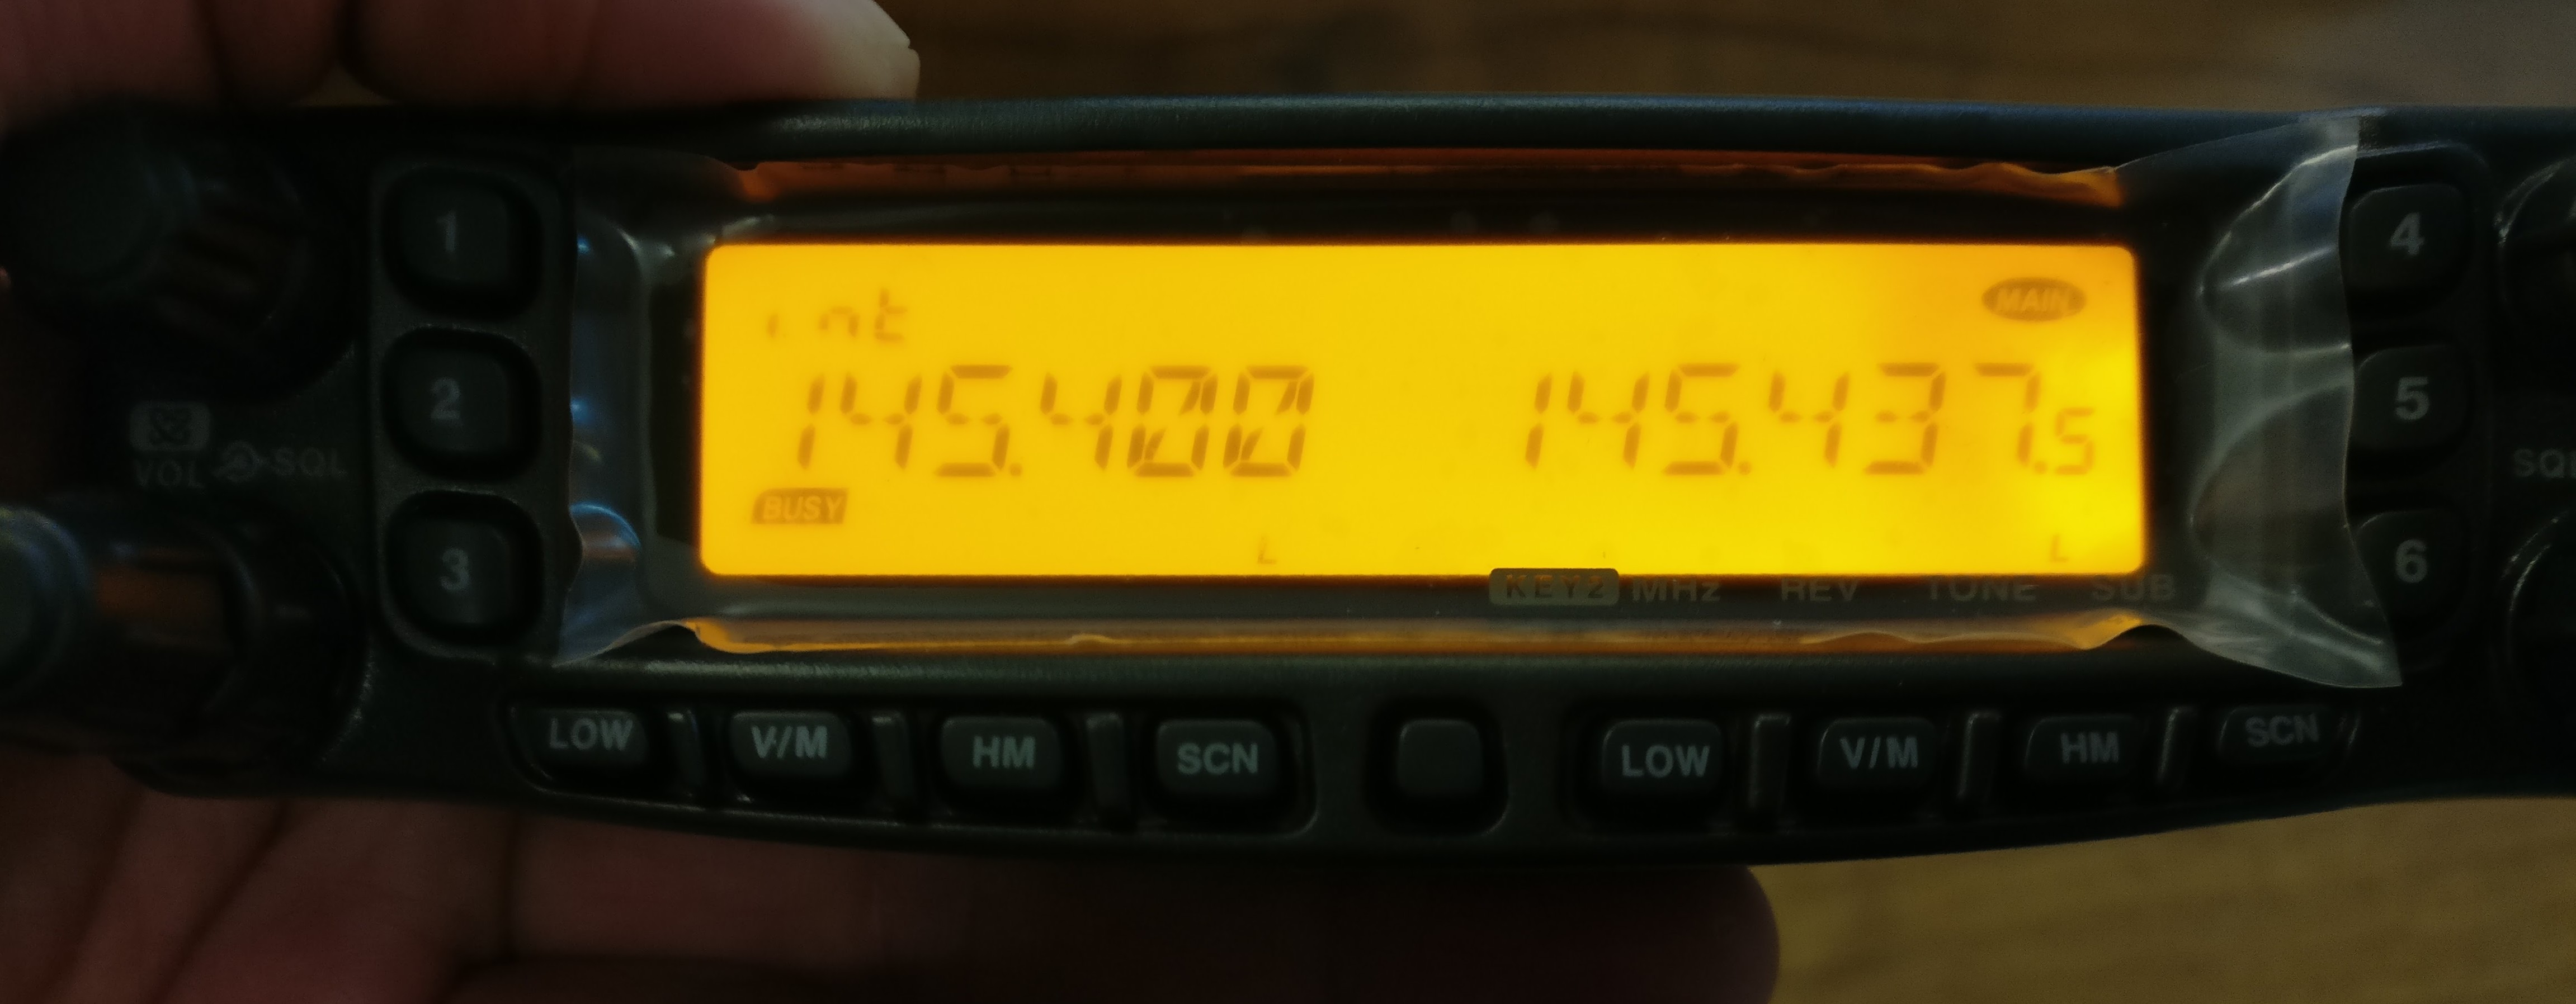
\includegraphics[width=1\textwidth]{img/radio_head}
    \caption[Picture of RT-8900r radio]{A picture of the face of the RT-8900r radio.}
    \label{fig:radio_head}
\end{figure}

The \gls{8900} (Seen in figure~\ref{fig:radio_head}) is a popular, budget amateur radio, it is marketed for mobile applications such as being mounted on a car dashboard. This is achieved using a control surface (hereby referred to as the head) that is detachable from the rest of the body of the radio. This allows the body to be mounted in a more practical location by running a control cable between the two. The \gls{8900} is capable of monitoring two separate frequencies at the same time, therefore there are duplicate controls on ether side of the radio to manipulate each receiver. The microphone connects into head and contains additional buttons such as a keypad that is able to dial a exact frequency. Conversely the loudspeaker is located in the body of the radio so a second cable must be run from the line out jack at the back of the radio to the head in order to hear audio clearly.

The main goal of this project is to allow the functions of the radio to be available from a computer. This will be achieved by adapting the \gls{8900} to have \gls{cat} features. Radios that come with this feature typically have a serial port or some kind. My project relies on the assumption that it is possible that the control line can be intercepted and emulated by a computer. This means that functionality could be added in a similar way to radios that advertise the C.A.T feature. This must be achieved cost effectively and in a simple way for the user to create and setup by themselves. Any designs and software will then be released under the GNU Public Licence (v3) for the benefit of the community.
\chapter{Problem analysis \& Objectives}
\section{Analysis}
After confirming the data port on the back of the device did not provide enough control \footnote{The data port only allows input and output of audio, transfer of station memory when the radio is in a special mode and control of squelch level.}, it became clear that the only way to interface with the radio without opening up the case (and invalidating the warranty) was to utilise the serial line that connects the head and body of the radio.

Previous work on understanding the serial protocol between the body and head of the radio was undertaken and compiled by Ben Cooper \cite{ben_report}\cite{8800r_reverse}. This work helped to ascertain the basics of the serial communication. Ben Cooper's project was focused on developing software aimed to run on a Arduino microcontroller. He concludes that the severe complexity of sending, receiving and processing on a single thread was perhaps reason to consider other options.

Considering the application may need to be run in these remote shacks with limited power and Internet connectivity. The project will aim to be as power and memory efficient as possible, so that it can be run on low specification hardware. This gives the benefits of a lower cost. Additionally for this reason the application must be portable for at least the x86 and ARM architectures so that it is actually possible to run on a low spec machine. This will give the user as many options as possible, for example low power PCs such as the Raspberry Pi or to just control the radio straight from a laptop that has serial capabilities. Development of the project will also benefit as common laptop/desktop hardware can be used with the use of a USB \gls{ttl} dongle. These dongles are cheap and ubiquitous, often costing less than \pounds1 each. This gives a low barrier to entry as it is the only dedicated hardware required for most users.

\subsection{Protocol}
Most of the protocol was already reverse engineered by other authors such as Ben Cooper~\cite{ben_report}, these assumptions were confirmed using a digital oscilloscope by being able to decode both \gls{tx} and \gls{rx}. Figure~\ref{fig:circuit_diagram} shows a circuit diagram, the connectors at each end of the circuit are RJ25 ports (aka telephone jacks) with 6 active lines. In the order of left to right from the perspective of looking into the socket, the first 2 lines are for \gls{rx} and \gls{tx} of serial, ground, 9v power, power switch and the last line is for the microphone. The radio does not use the common RS232 standard\footnote{RS232 sends binary with -13V to represent a one bit and +13v for a 0 bit, allowing for easy knowledge of when the line is idle at 0V} instead it uses the older \gls{ttl} standard. In this case this means that an idle line is at 5V which represents a 1 bit and 0V representing 0 bit. The beginning of a transmission is marked with a single start bit, followed by 8 bits of data and then a single stop bit. There is no error checking through parity or otherwise. 

So to summarise the communication: 
\begin{itemize}
    \item 0-5V
    \item \gls{ttl} protocol
    \item 8 data bits with 1 stop bit
    \item The most significant bit is transferred first
    \item 19,200 baud rate
    \item Automatic shutoff after 80ms
\end{itemize}

\gls{tx} from the head to the body of the radio does two things. For analogue buttons it transmits the current state of those buttons and for digital encoders, such as the dials, it transmits the number of rotations since the last \gls{tx}. The packet of data that is sent consists of 13 bytes (mapped previously\cite{ben_report}). This could be utilised as a method to provide emulated input to the radio. Actions could be undertaken by the program to replicate any input that a human was capable of.

\begin{figure}
    \centering
    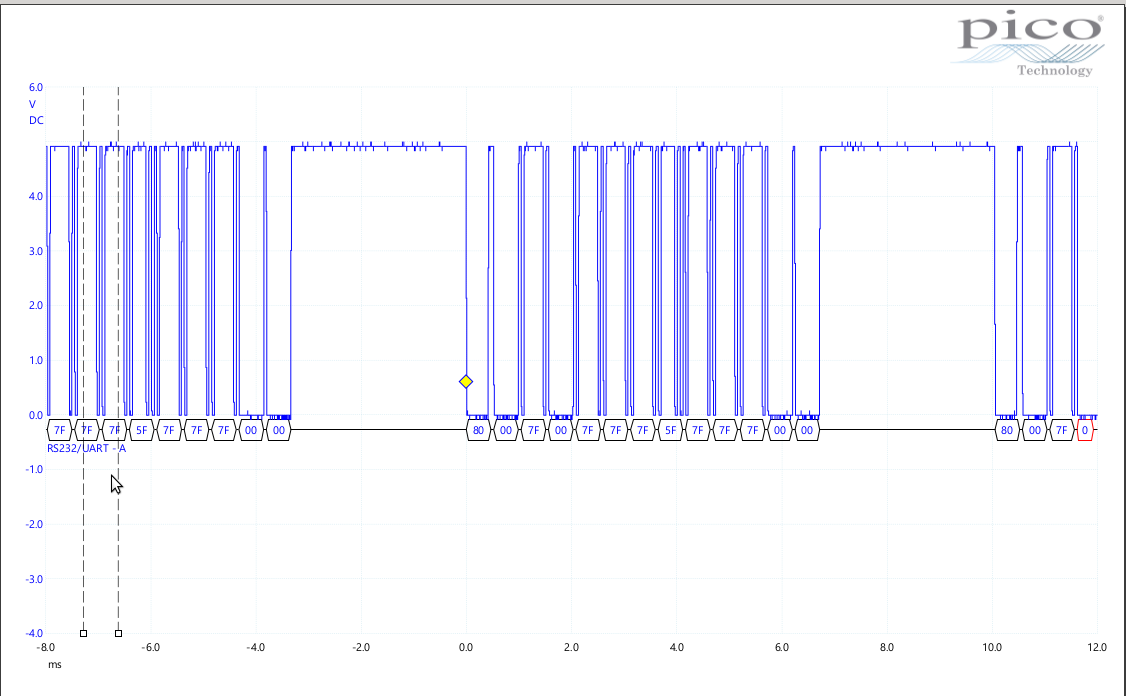
\includegraphics[width=1\textwidth]{img/controll_packet.png}
    \caption[Control packet]{A capture of control packets. The 2 long peeks are the begging and end of the middle packet}
    \label{fig:control_packet}
\end{figure}

\gls{rx} (from the body to the head) is a packet of 42 bytes. Each bit in the packet represents whether a segment of the screen should be illuminated or not, for example what frequency should be shown. The program can listen to this to learn the internal state of the radio. The state of the radio that is not represented on the screen will have to be discovered by navigating the menus and then reading the screen.

During the project there where some new observations made to the transmission protocol. The most significant bit (MSB) is transmitted first between the radio and head with a 20ms gap between both \gls{rx} and \gls{tx} packets. The head will transmit its \gls{tx} packets as soon as it is given power if the body is given the boot signal (setting the 5th line to low) but without receiving head packets it will shutdown after 80ms. The only indication of this boot failure is is a small audible click sound from the loudspeaker. 

\section{Aim \& Deliverables}
The scope of development efforts will be to create a way to control the body of the radio, with the aim to achieve as much functionality as possible (controllable by a computer). Communication to the head, for the purposes of using it as a generic control surface will remain out of scope. This non-critical feature would be at a high cost in time spent, when instead more important control features could be implemented. However work done that is in scope will be foundational to this feature if desired later. Dealing with the audio from the radio was also deemed out of scope, as the data-port of the back of the radio can already achieve this. Users can use a cable speaker line out and microphone line out from the back data port.

Below is a list of deliverables. Necessary functions were derived by asking a number of ``Customers'' what they would consider their minimum set of features (aka the planning game) and there expected difficulty. They are also in order of priority. Therefore this became the priority backlog.

\begin{itemize}
    \item Final report
    \item Software functions that have been deemed necessary for radio control:
        \subitem Frequency
        \subitem Push to talk
        \subitem Volume
        \subitem \gls{squelch}
        \subitem Power
        \subitem Powering on the radio
    \item Documentation
        \subitem Code documentation (\gls{doxygen})
        \subitem Schematic of prototype serial controller
\end{itemize}

Futures such as a more permanent printed circuit board and control of all functions of the radio were deemed not possible in the allotted semester of work\footnote{From \formatdate{30}{01}{2017} to \formatdate{08}{04}{2017}.}. Originally there was expressed intent on providing a patch to the open source Ham Radio Control Libraries, Hamlib\cite{hamlib}. The Initial report outline submitted reflected this. However after discussion of this intent on the developer mailing list it became clear that a multi-threaded application was unacceptable within the Hamlib codebase, due to concerns with portability and stability. Instead future work will likely include some sort of inter process communication through a socket.

\section{Security}
The envisioned scope of the project means that the software will not be networked in the modern sense of using IP communication. If the project did so there would be many security issues raised in how connections are handed, what kind of authentication is used and how will traffic be encrypted. Major operating systems manage access to serial communications often by requiring special privileges or groups. Therefore in this case, loss of access control can be prevented using just the default system configuration of most operating systems. The application will endeavour to not manipulate the system as much as is possible so as to minimise the attack surface given. Attention will be given to proper copying in memory and validation of incoming received serial communications to mitigate fuzzing based attacks.

Considerations must be made on who has physical access to the computer connected to the radio. As another user could plug the serial connection into their computer in order to interface with it, thereby forgoing the access control that was in place on the system. Users will also have to consult their local laws on whether it is legal for them to operate their radio remotely in their respective countries. 

\section{Process}
Due to the large potential scope of the project it was necessary to choose an agile methodology so that the large set of possible requirements could be better managed and prioritised. Therefore agile software development methodologies had to be constituted and chosen on their merit for the project. Methods considered were Scrum, \gls{xp} and \gls{fdd}. \gls{fdd} was quickly ruled out due to its major benefits only seen with larger teams that need to be able to produce regular status reports. For this project it was feared this would slow down the rate of development of features. Scrum was seen as less useful than \gls{xp} as it does not talk about the actual engineering steps to take in programming unlike \gls{xp}. Instead it focuses more on general management for a team. Therefore \gls{xp}\cite{extreme_programming} was chosen, however it still had to adapted for a single person project.

\gls{xp} guidelines for design can be summarised to the following\cite{xp}:
\begin{itemize}
    \item The Planning Game
    \item Small Releases (Iterations)
    \item System Metaphors
    \item Simple Design 	
\end{itemize}

\begin{figure}
    \centering
    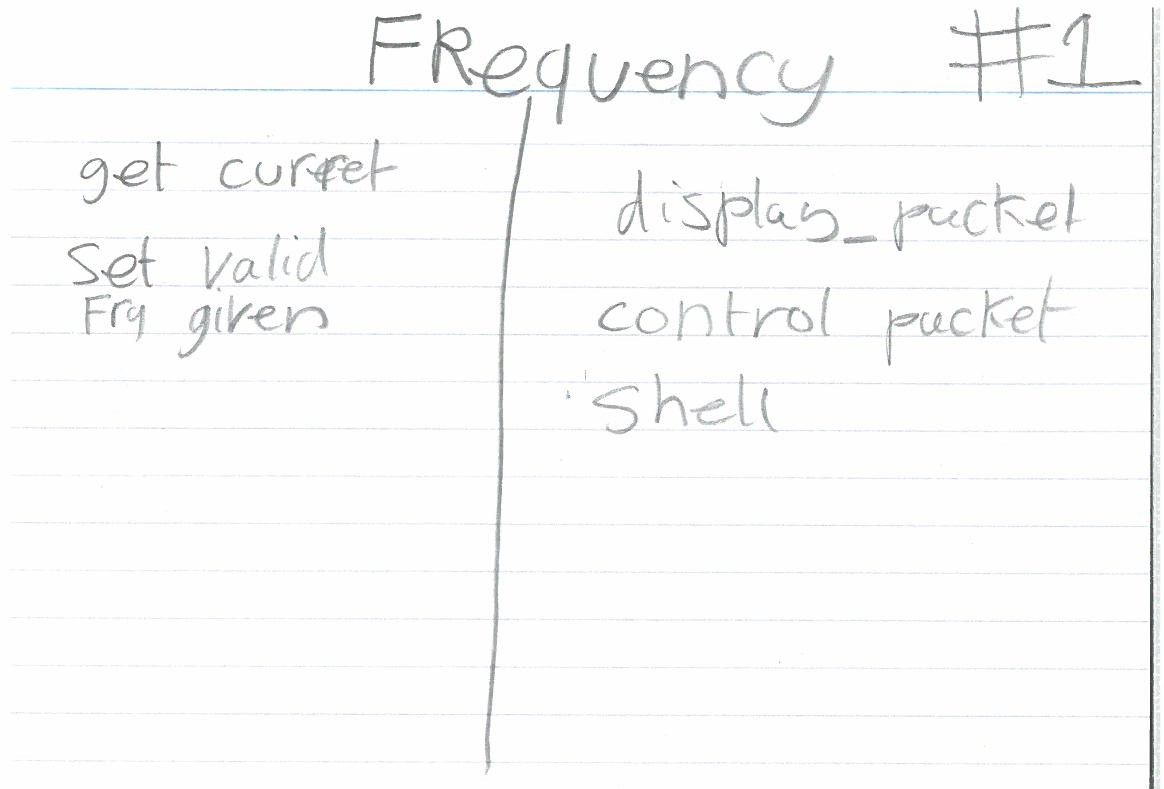
\includegraphics[width=0.5\textwidth]{img/crc_front}
    \caption[CRC front]{The front of the CRC cards contained on the left the required functions of the feature and what it will deal with on the right.}
    \label{fig:crc_front}
\end{figure}

\begin{figure}
    \centering
    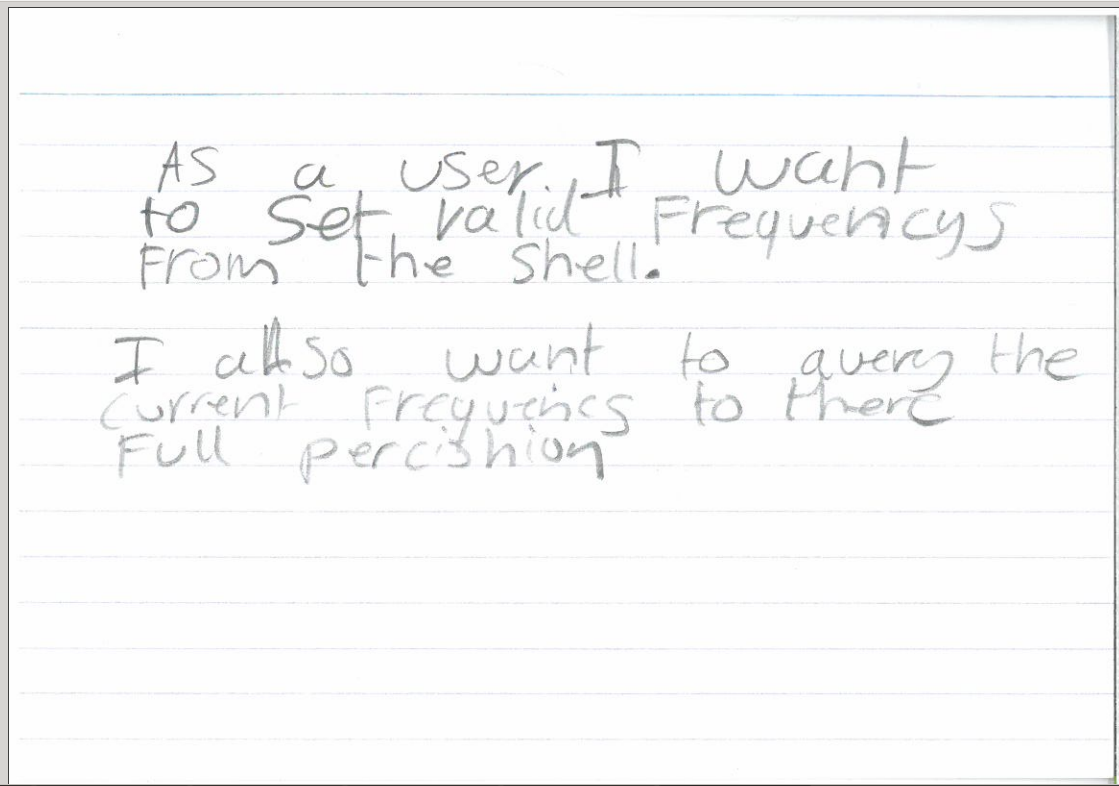
\includegraphics[width=0.5\textwidth]{img/crc_back}
    \caption[CRC back]{The back of the CRC cards contained the acceptance tests for the feature.}
    \label{fig:crc_back}
\end{figure}

The above points are very compatible for a lone developer project. The planning game was used with potential ``customers'' (Customers were any potential user of the radio i.e with the project supervisor), by requesting features to be prioritised. This was then used to produce and sort \gls{crc} cards (See figures ~\ref{fig:crc_front} and \ref{fig:crc_back} for the front and back of a \gls{crc} card respectively). Use of system metaphors was fairly common when discussing the project, this can been seen in this report with the ``head'' and ``body'' metaphors and standardisation of point of reference to serial communication with the \gls{rx}/\gls{tx} terms. Small releases at the end of each iteration were make allowing users give regular feedback. The initial design of the application was made to be just large enough to start development without the need for heavy refactoring later.

The actual development methods used in \gls{xp} will need to be modified in order to accommodate one developer. Thankfully adaption to a single developer as been discussed openly, including from the creator of \gls{xp}, Kent Beck in a number of mailing list discussions\cite{xpforone}\cite{lone_developer}.

The following sections will address the adaptations made:
\subsection*{Unit Tests}
The described use of unit tests do not need to be changed for the project. The test suite ``Google Tests''\cite{google_tests} was chosen despite the fact that this is implemented in C++, as it is often used to test C code and better support and features than native suites. Its test macros are familiar to programmers that have used suites such as JUnit etc. Unit tests were especially useful for the project as the real hardware was not always available for testing the radio was stored in a university lab that was shut on the evening, Fridays and weekends. 

\subsection*{Acceptance Tests}
Acceptance Tests are created on the back of \gls{crc} cards. A successful test is likely to be the ability for the user to preform said action on the real radio without any input from the developer. A passing acceptance test is the only verification of a completed feature.

\subsection*{Refactoring}
Refactoring should occur naturally throughout development as well as during the refactoring stage of creating a function with the \gls{rgf} method. Good use of unit tests will make refactoring easier as developers can make changes with confidence of not braking the system.

\subsection*{Pair Programming}
\gls{xp} has a heavy focus on pair programming. This project work is not permitted with other developers in order for a full assessment to take place of work done. Instead other methods that give some of the benefits of group collaboration such as``rubber ducking'' will be used. Rubber ducking is the process of talking out or explaining code to oneself in order to check that there are not better ways to do something. Throughout the project conversations with other students about the project, for example when walking up to campus was used to provide reflection. Questions from others asking why something was done in a particular way can often promote further analysis and better ideas.

\subsection*{Continuous Integration}
Git will be used as a VCS for the project using branches for new features before merging them, this was chosen over over VCS due to its better branching and mergeing as well as ability to still commit when disconnected from the Internet. Github will be used to host the central repository, due to its good user interface as well as its large popularity (meaning new user discovery is possible). A self hosted version of Jenkins\cite{jenkins} will used automatically test commits by running builds. Jenkins CI was chosen due to previous positive experiences with it as well as its high level of customisation owing to its large plugin library. 

\subsection*{Coding Standards}
The ``Linux kernel coding style''\cite{linux_coding_style} was chosen as it is a widely used standard that has a good rationale and format. To enforce a consistent style checking to was made in the text editor, as well as a step in continuous integration checks to look for style violations.

\subsection*{Iterations}
The project will run using two week iteration/release cycle. It is hoped that this will give enough time to plan, develop, and physically test the radio functions. In this time the current most needed feature from the priority backlog will be worked on. To do this a number of engineering tasks are made from the feature and placed as ``TODO'' items in the source code. This is the most appropriate place as tasks remain very visible until removed, unlike when tasks are recorded on a webpage elsewhere.  At the end of an iteration a release is tagged in git with a version number that conforms to the semantic versioning convention\cite{sem_ver}. Additionally a changelog is made on the developer blog. This means there are regular versions of the software that can be tested and reflections can be made about the progress of the project.

%\addcontentsline{toc}{chapter}{Development Process}
\chapter{Design}
\label{section:design}

% \todo[inline]{
% You should concentrate on the more important aspects of the design. It is essential that an overview is presented before going into detail.

% As well as describing the design adopted it must also explain what other designs were considered and why they were rejected.The design should describe what you expected to do, and might also explain areas that you had to revise after some investigation.

% Typically, for an object-oriented design, the discussion will focus on the choice of objects and classes and the allocation of methods to classes. The use made of reusable components should be described and their source referenced. Particularly important decisions concerning data structures usually affect the architecture of a system and so should be described here.How much material you include on detailed design and implementation will depend very much on the nature of the project. It should not be padded out. Think about the significant aspects of your system. For example, describe the design of the user interface if it is a critical aspect of your system, or provide detail about methods and data structures that are not trivial. 

% Do not spend time on long lists of trivial items and repetitive descriptions. If in doubt about what is appropriate, speak to your supervisor. You should also identify any support tools that you used. You should discuss your choice of implementation tools - programming language, compilers, database management system, program development environment, etc. Some example sub-sections may be as follows, but the specific sections are for you to define. 
% }
\section{Hardware}
\begin{figure}
    \centering
    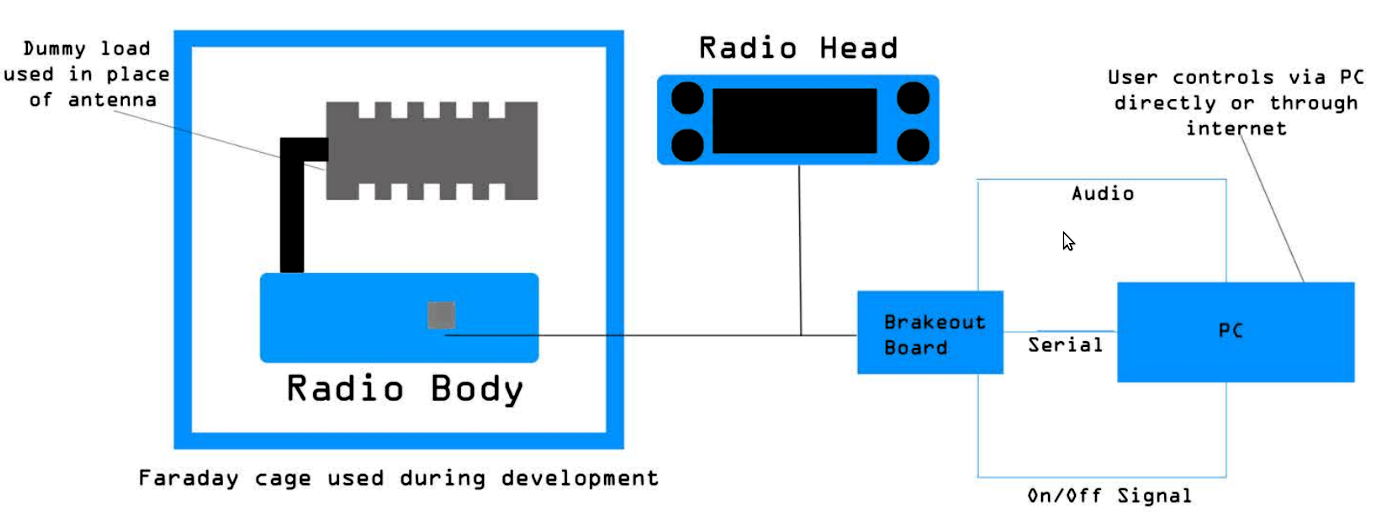
\includegraphics[width=\textwidth]{img/setup_diagram}
    \caption[Hardware Overview]{A hardware overview of the project.}
    \label{fig:setup_diagram}
\end{figure}

\begin{figure}
    \centering
    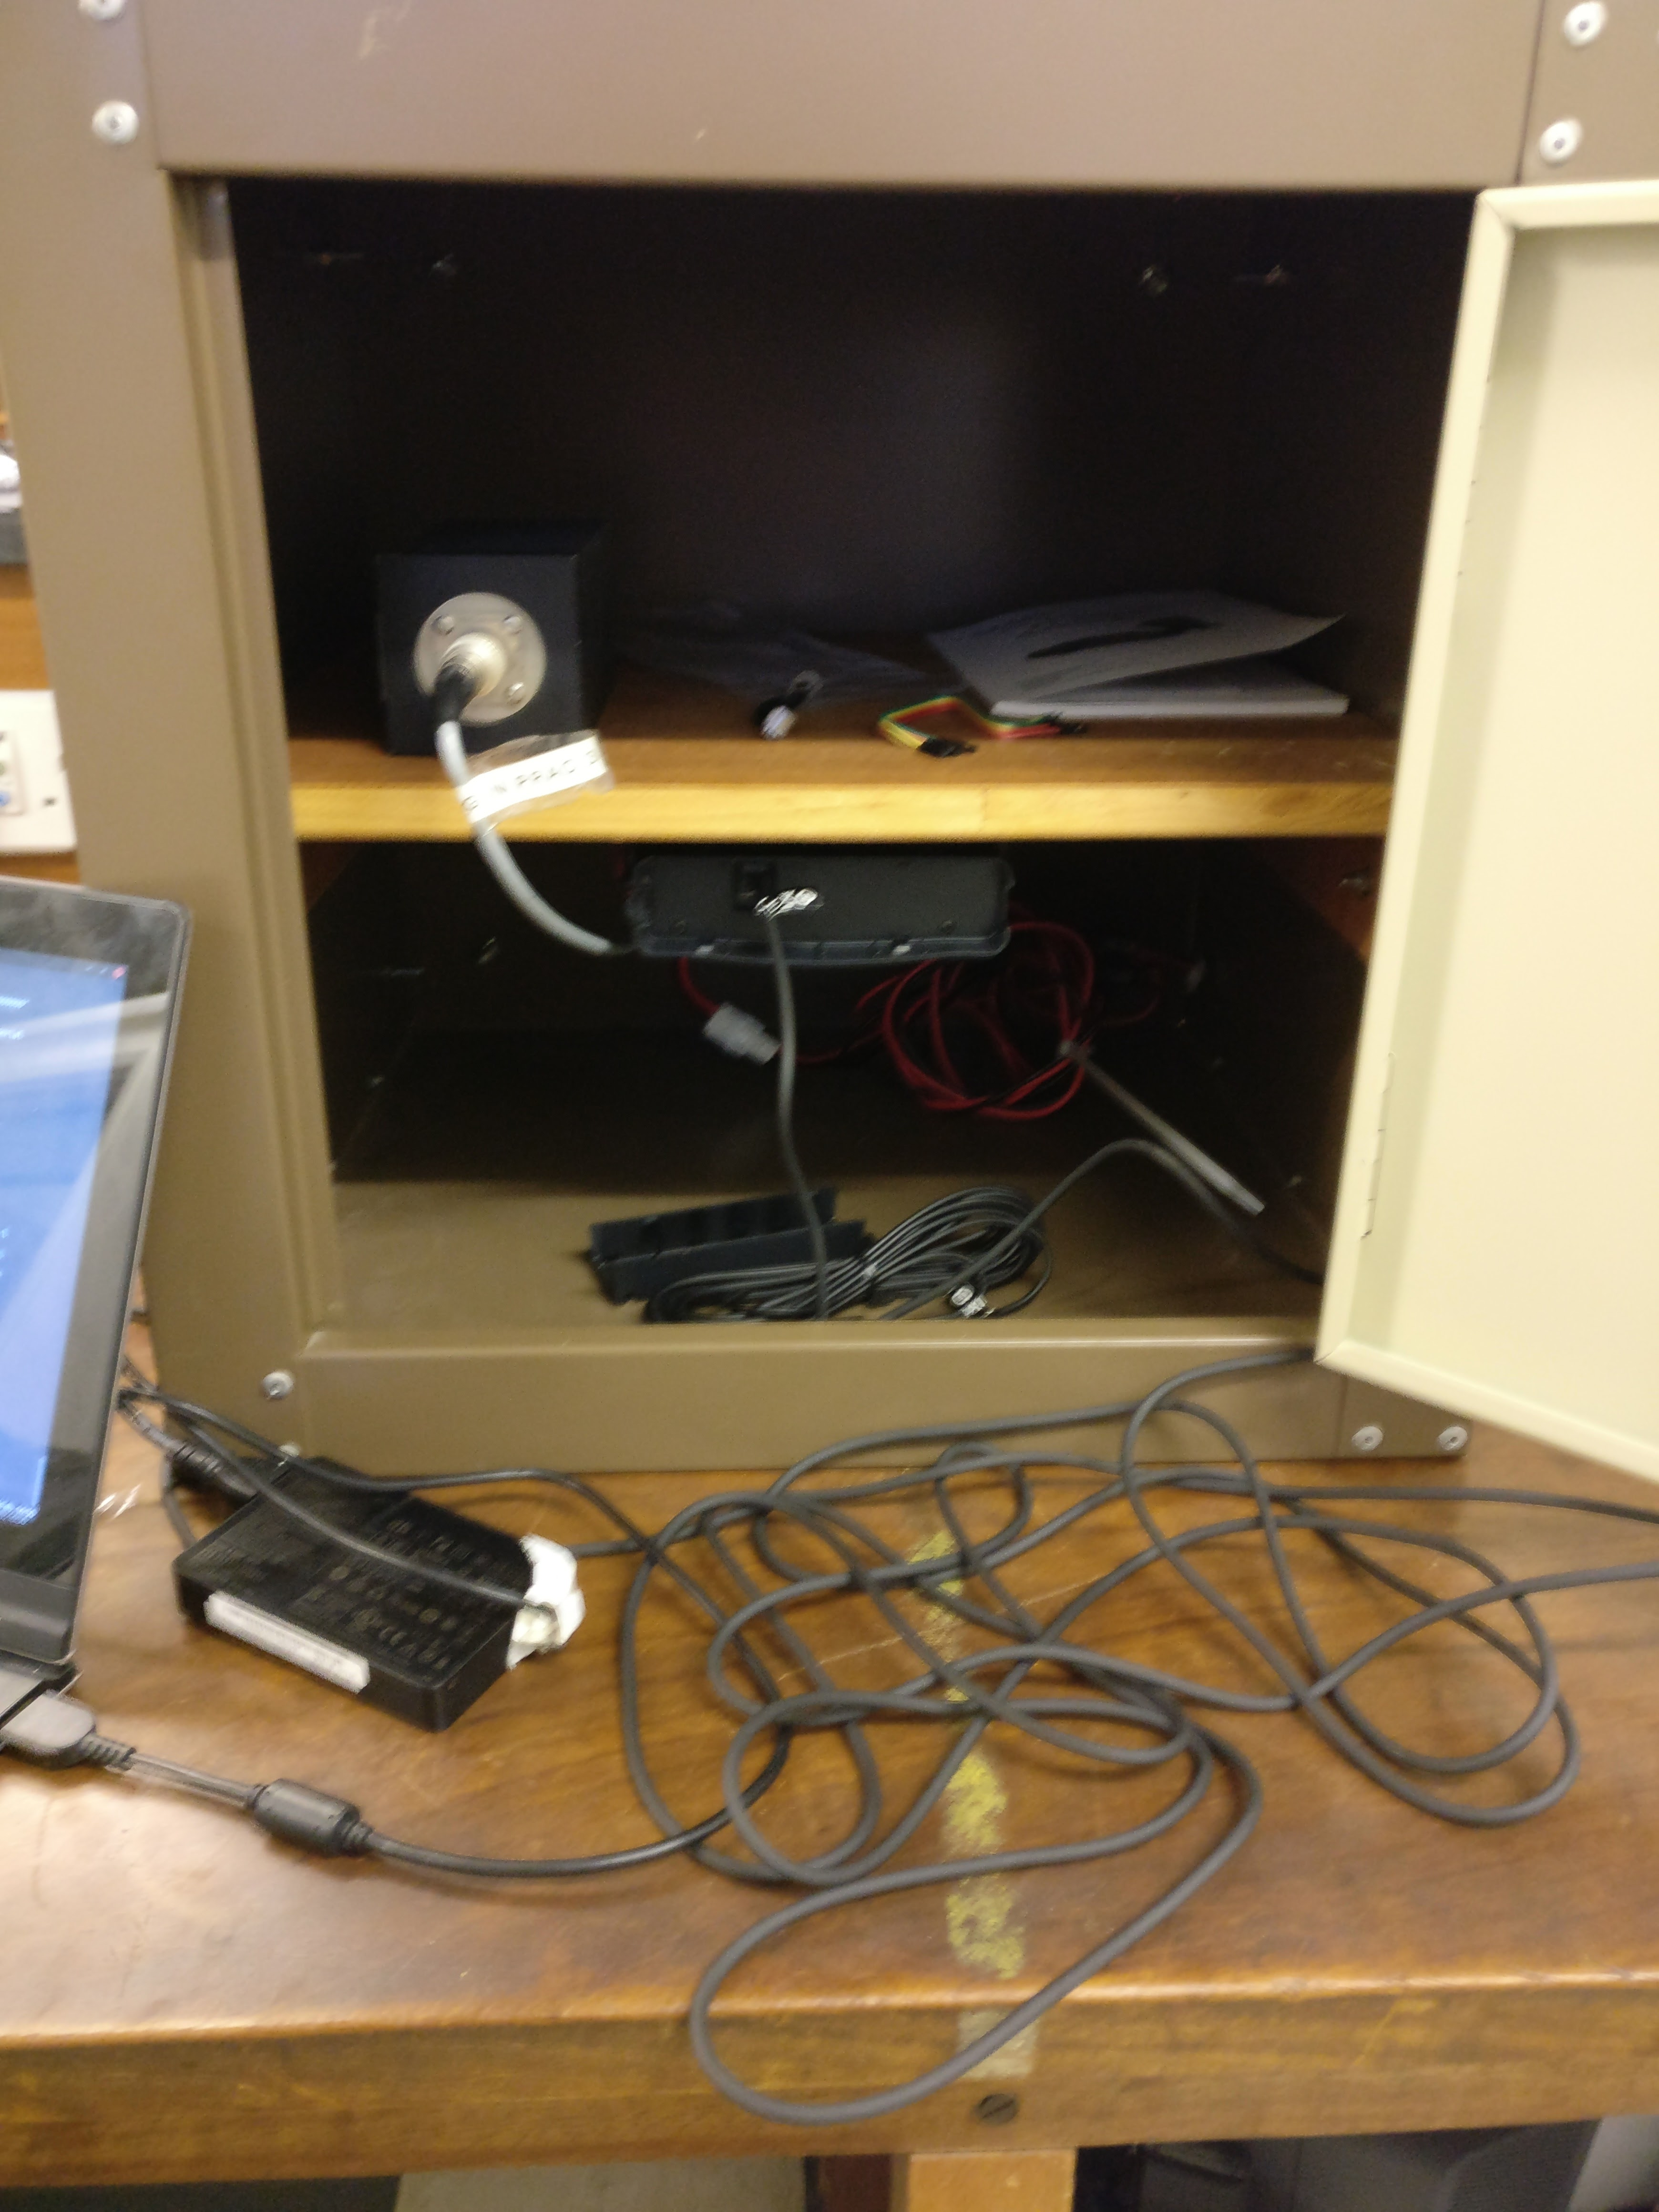
\includegraphics[width=0.5\textwidth]{img/locker.jpg}
    \caption[Radio locker]{A picture of the metal locker used to contain radio waves made from the radio body. The black box below the wooden shelf is the radio body. The box above is the dummy load.}
    \label{fig:locker}
\end{figure}

In order to develop software for the radio, it had to be ensured during development that an error in the program did not lead to rouge transmissions. To do this the radio was suspended on a wooden shelf placed in a grounded metal locker (See Figure~\ref{fig:locker}). Connected to the radio was a dummy load in place of aerial, with power to the radio coming through a whole in the side of the locker so that the door could remain closed. This helped to reduce the strength of any transmissions significantly but not entirely. As a final precaution a second hand-held radio was placed next to the \gls{8900} to monitor for any transmissions. If this was to occur the developer could then shutdown the radio quickly so as to avoid prolonged transmission.

\begin{figure}
    \centering
    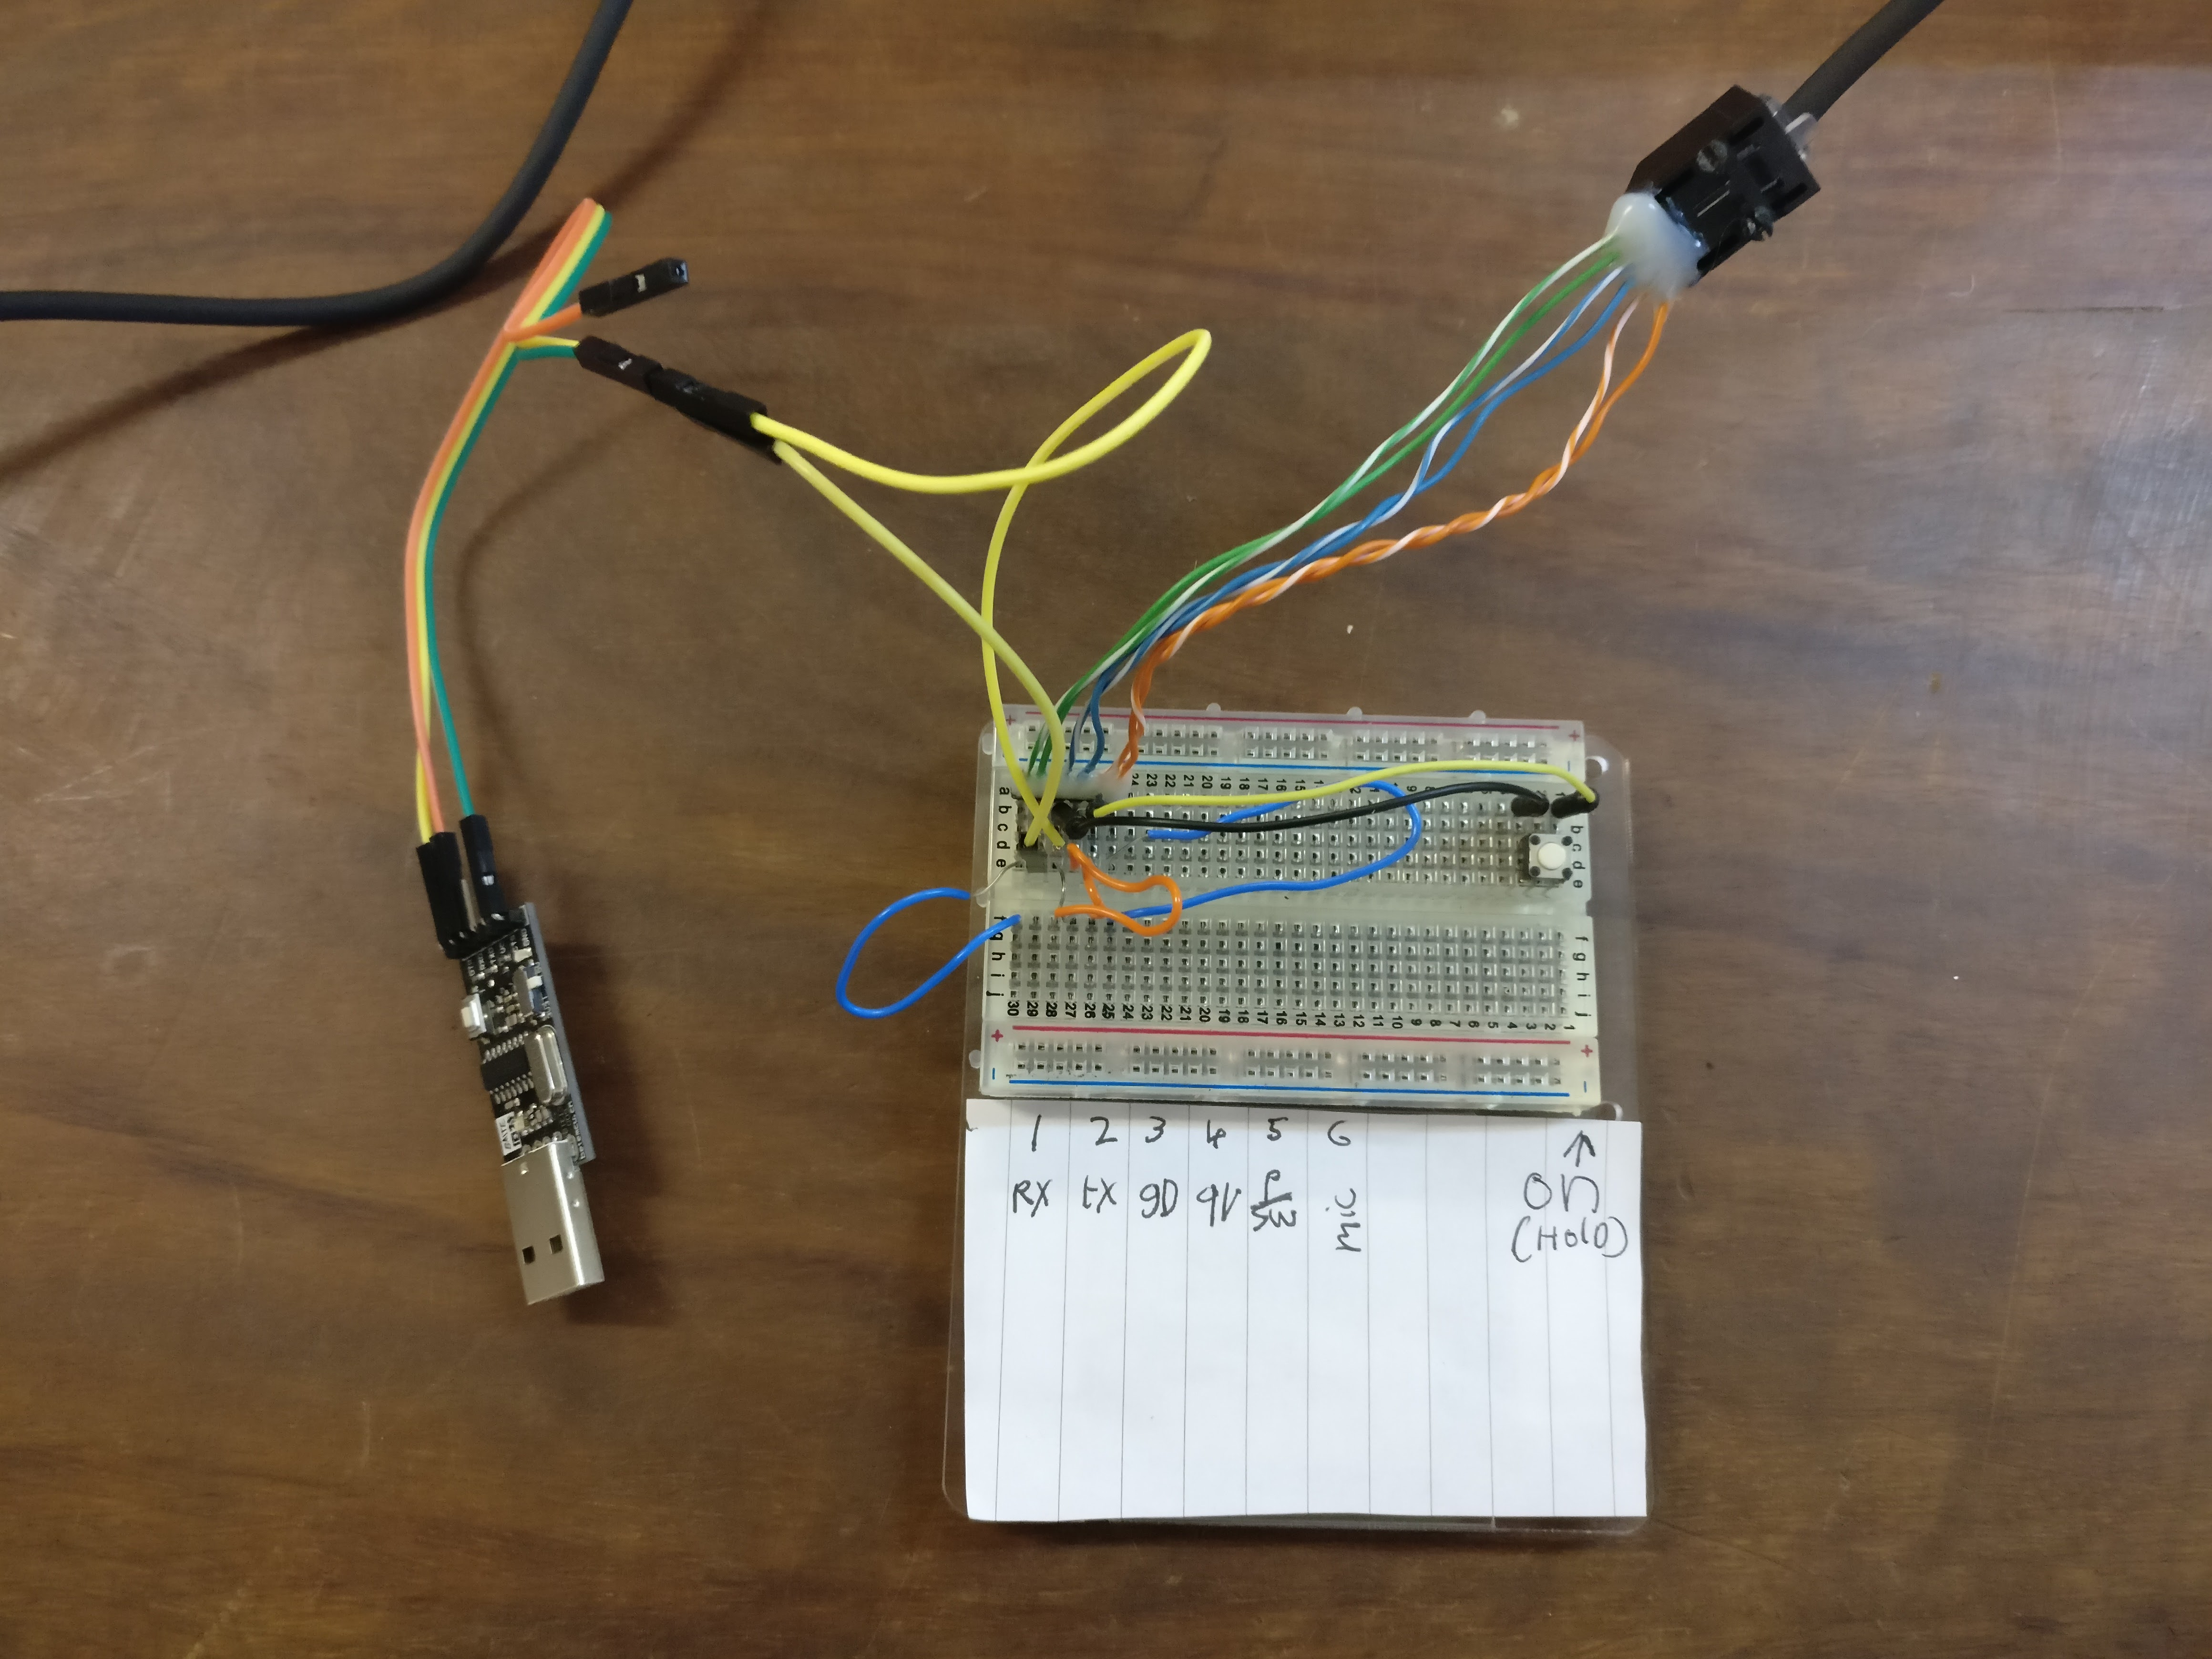
\includegraphics[width=0.9\textwidth]{img/bread_board}
    \caption[Prototype breakout board]{Prototype breakout board used for development.}
    \label{fig:brake_out_board}
\end{figure}

The serial brake-out board (shown in figures~\ref{fig:brake_out_board} and \ref{fig:circuit_diagram}) passes though the required connections to the head of the radio. Allowing the head to still be used, even when the body is controlled by the radio. The ground, \gls{rx} and \gls{tx} serial connections are tapped by the serial dongle with the \gls{tx} being the only disconnected line from the radio. There is also a physical button that connects the power switch to ground when pressed, effectively having the same effect as pressing the power button on the head of the radio.

\begin{figure}
    \centering
    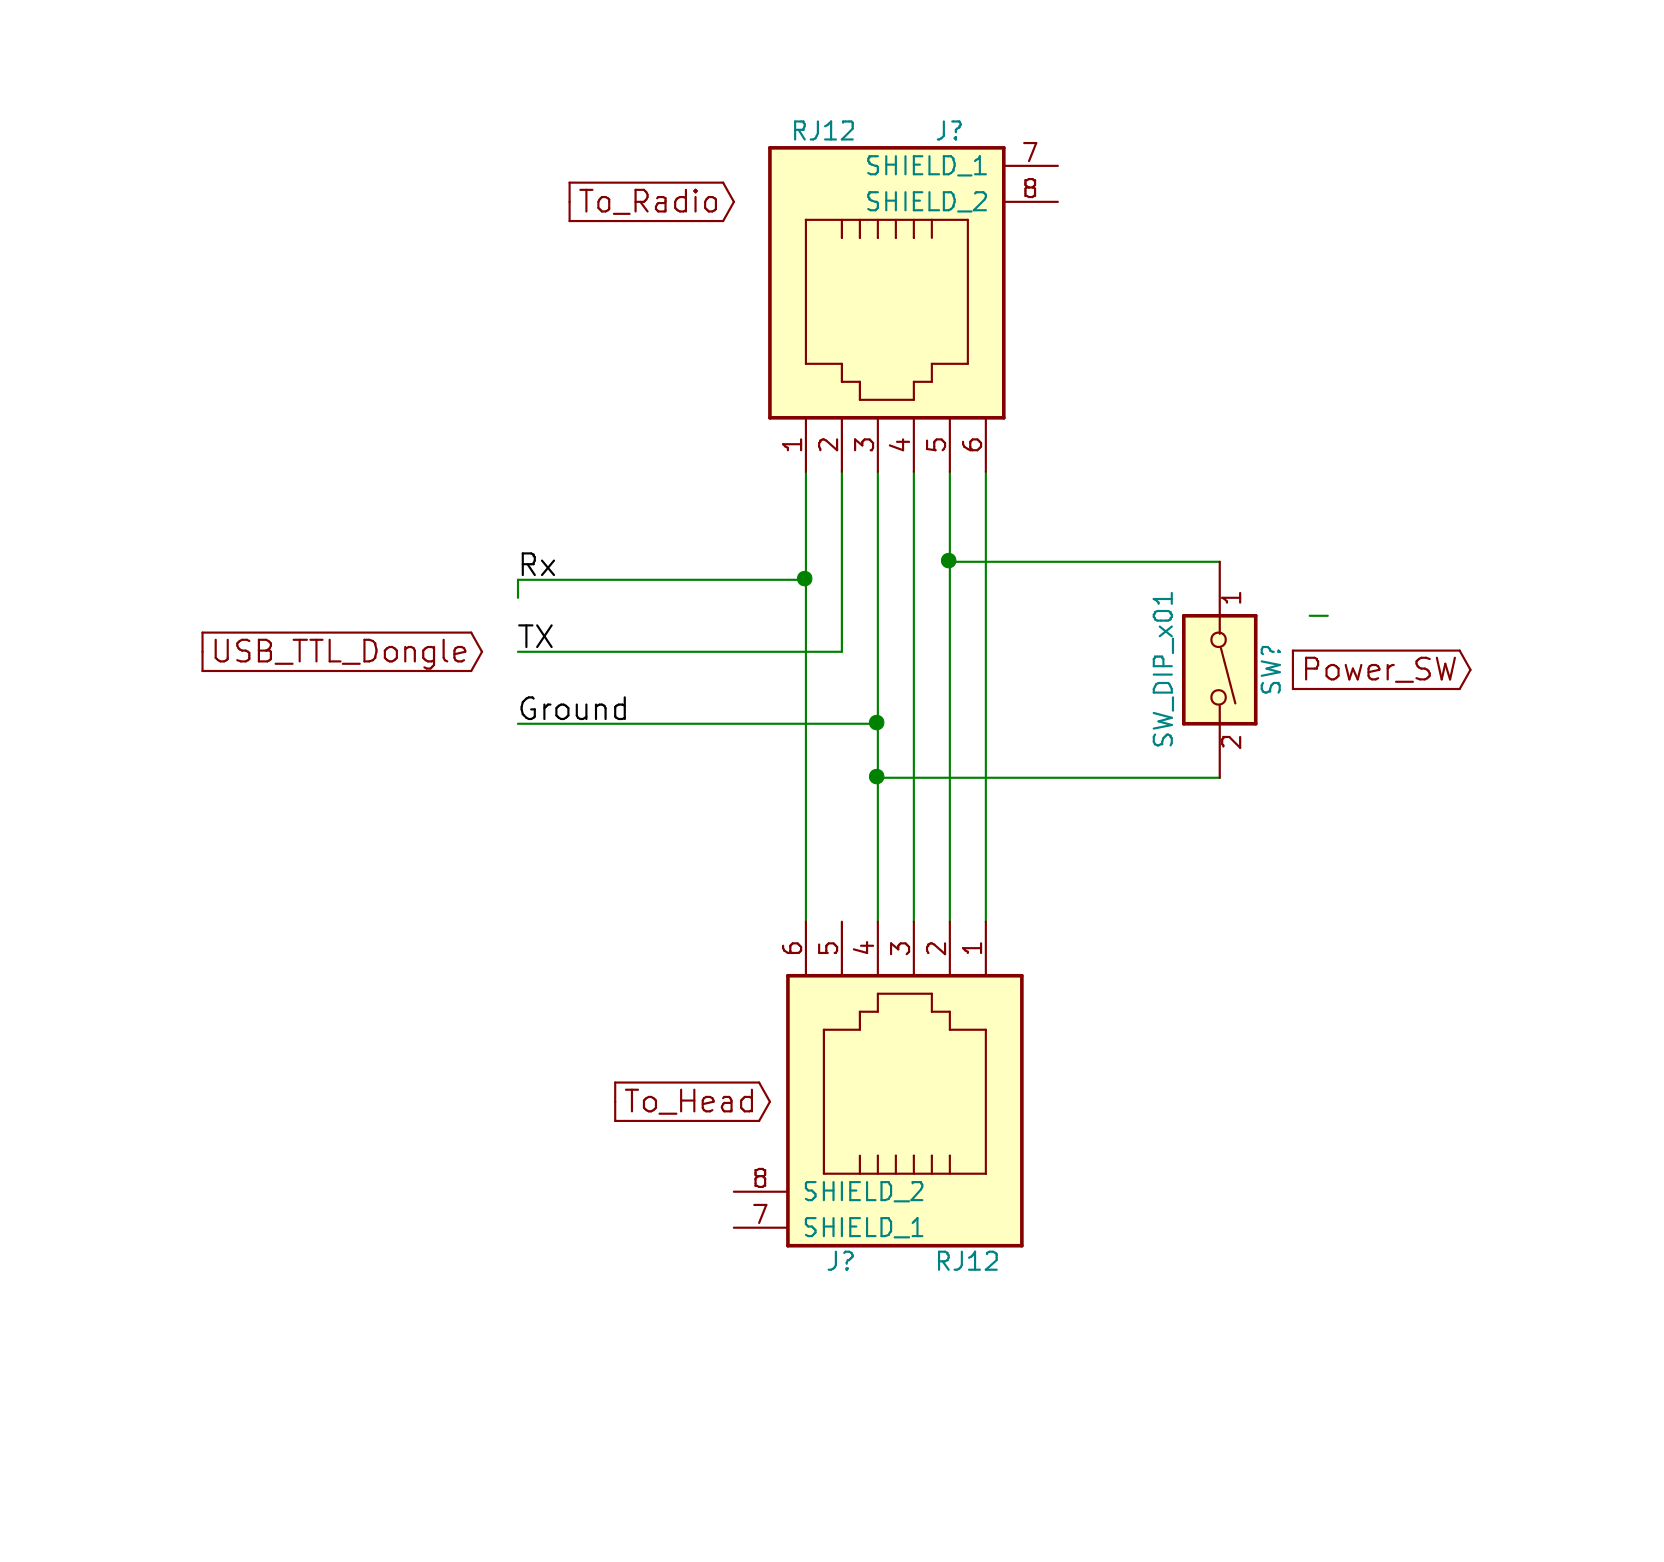
\includegraphics[width=\textwidth]{img/circit.png}
    \caption[Circuit diagram]{Circuit diagram of the brake out board}
    \label{fig:circuit_diagram}
\end{figure}

\section{Overall Architecture}
The more generic functions of the application will be abstracted out to a library so that they can be reused within other applications. The application will provide a console or shell for the user to control the radio from. A console is an appropriate interface as the \gls{xp} methodology demands that designs be made as simple as possible, while still satisfying acceptance tests. Another reason is that the program will ultimately be, an intermediary for signals and not the primary way for the user to control the radio. This is due to the large number of existing and successful free radio control applications designed for such a purpose; for example GRig\cite{grig}. 

\begin{figure}[H]
\centering
    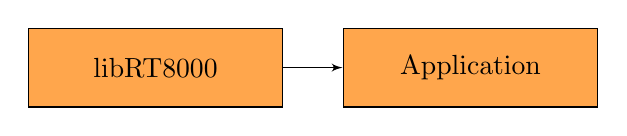
\begin{tikzpicture}[node distance=2cm]
    \node (lib) [process] {libRT8000};
    \node (app) [process, right of=lib, xshift=2cm] {Application};
    \draw [arrow] (lib) -- (app);
    \end{tikzpicture}
    \caption[basic architecture]{The basic overall library/application architecture}
\end{figure}

The the radio must receive packets every 80ms, else it will automatically shutdown. With such a time critical task such as this, the routine was given a separate thread to operate in, so as to lower the impact of other routines on its timing. This is described in figure~\ref{fig:sender_thread}. 

\begin{figure}[ht]
\centering
    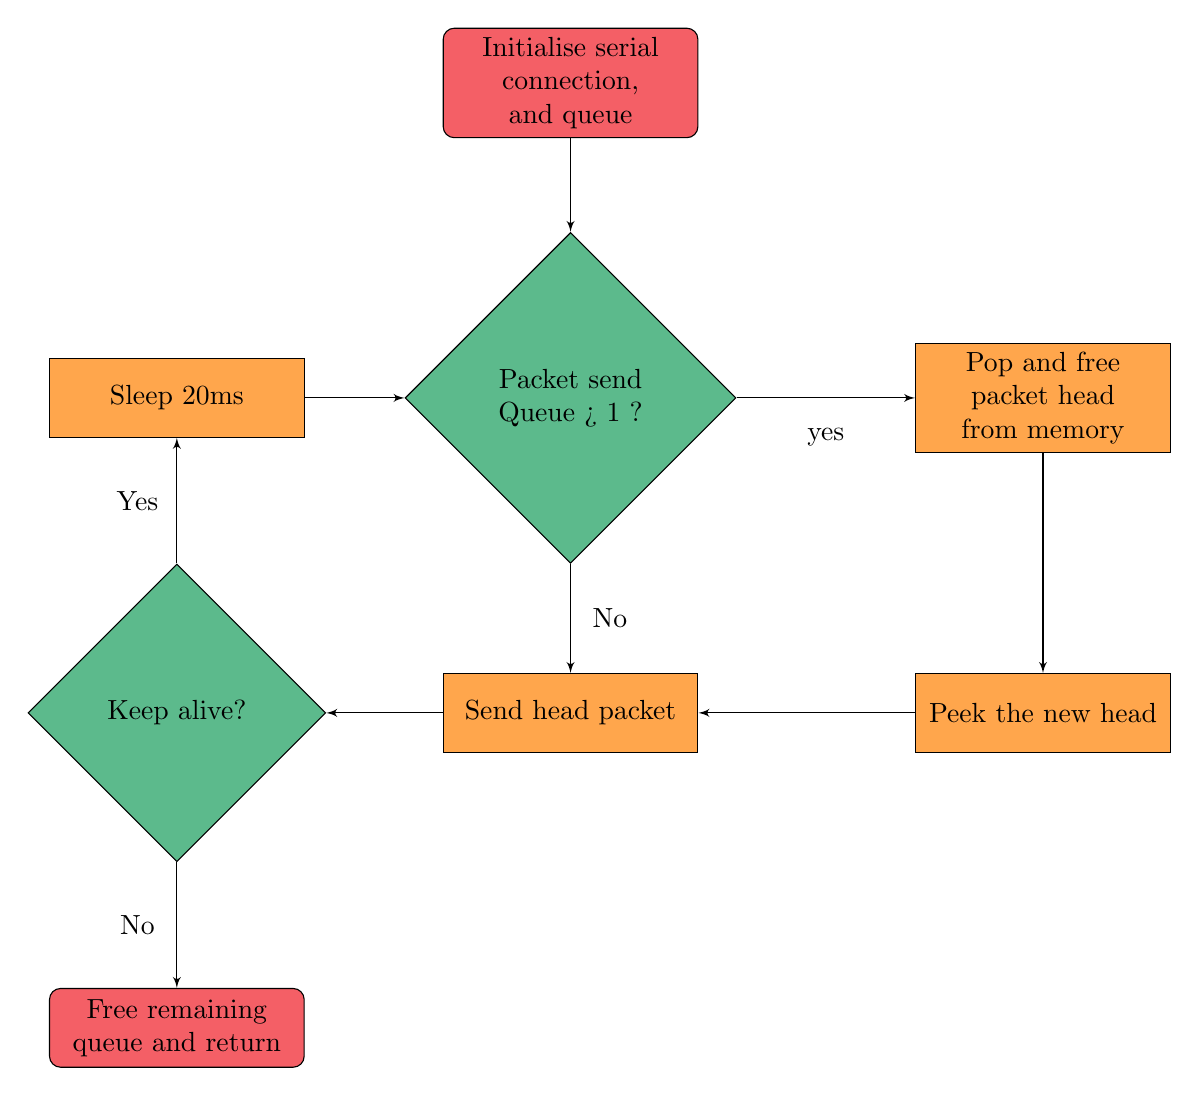
\begin{tikzpicture}[node distance=2cm]
% decision, right of=lib, xshift=2cm
    \node (checkq) [decision, xshift=-4cm] {Packet send Queue > 1 ?};
    \node (start) [startstop, above of = checkq, yshift=2cm] {Initialise serial connection, and queue};
        \draw [arrow] (start) -- (checkq);
    
    \node (pop) [process, right of=checkq, xshift=4cm] {Pop and free packet head from memory};
        \draw [arrow] (checkq) -- node[yshift=-0.5cm]{yes}(pop);
        
    \node (peek) [process, below of=pop, yshift=-2cm] {Peek the new head};
        \draw [arrow] (pop) -- (peek);
    
    \node (send) [process, below of=checkq, yshift=-2cm] {Send head packet};
        \draw [arrow] (checkq) -- node[xshift=0.5cm]{No} (send);
        \draw [arrow] (peek) -- (send);
        
    \node (shutdown_q) [decision, left of=send, xshift=-3cm] {Keep alive?};
        \draw [arrow] (send) -- (shutdown_q);
        
    \node (shutdown) [startstop, below of = shutdown_q, yshift=-2cm] {Free remaining queue and return};
        \draw [arrow] (shutdown_q) -- node[xshift=-0.5cm]{No} (shutdown);
        
    \node (wait) [process, left of=checkq, xshift=-3cm] {Sleep 20ms};
        \draw [arrow] (shutdown_q) -- node[xshift=-0.5cm]{Yes} (wait);
        \draw [arrow] (wait) -- (checkq);
    
    \end{tikzpicture}
    \caption[Sender thread]{Flow diagram of the Sender thread}
    \label{fig:sender_thread}
\end{figure}

Items in the queue are only removed (popped) when there is more than a single packet inside. This is done in order to prevent the automatic shutdown of the radio. The effect is that the last packet is kept in the queue and resent continuously until a new packet is added or the program shutdown. 

While designing the packet sender thread the idea of the ``default packet'' was imagined. This packet will contain much of the state of the radio. To change the volume the default packet is directly modified. More complex actions, for example actions that require a button to be pressed only momentarily, will add new packets to the queue. As there will possibly be duplicate packets in the queue, the queue implementation must hold only a reference to the default packet.

It was anticipated that the bulk of memory usage will be to store representations of packets. Therefore the data structure should be as memory efficient as possible. Although this must balance with the ease of use i.e sections being able to be mapped accordingly. Packets are to be stored as a bitfield. This is so that the \gls{rx} packet will take up only 42 bytes (or as close to this as possible). Bit-wise operations would then be used to read and set bits inside the packet. This has the added benefit that sending via serial will not require any additional processing, as the representation is identical.

Packets sent to the screen (\gls{rx}) will hereby be referred to as ``display packets''. These are used to generate the output of the display, where a set bit in the packet corresponds to an illuminated segment on the display. The packets that are \gls{tx} to the radio body will be referred to ``control packets'' as they communicate the current state of the controls back to the radio.

\begin{figure}[H]
\centering
    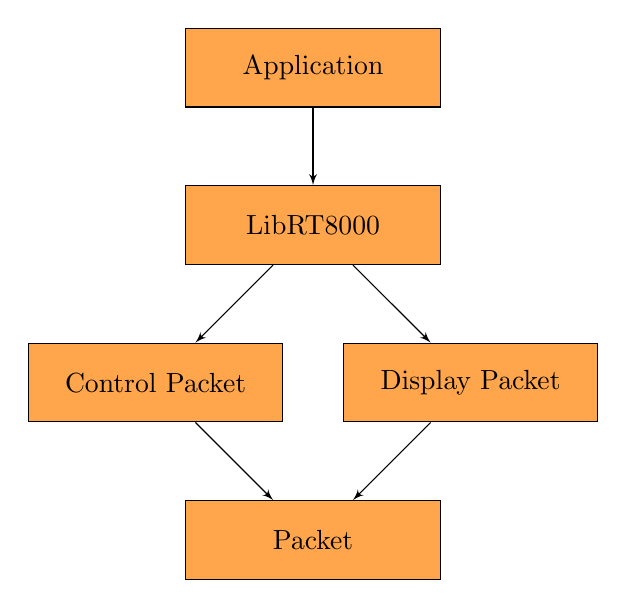
\begin{tikzpicture}[node distance=2cm]
    \node (app) [process] {Application};
    \node (lib) [process, below of=app] {LibRT8000};
        \draw [arrow] (app) -- (lib);
        \node (control) [process, below of=lib, xshift=-2cm] {Control Packet};
        \node (disp) [process, below of=lib, xshift=2cm] {Display Packet};
        \draw [arrow] (lib) -- (control);
        \draw [arrow] (lib) -- (disp);
            \node (packet) [process, below of=disp, xshift=-2cm] {Packet};
             \draw [arrow] (control) -- (packet);
             \draw [arrow] (disp) -- (packet);
    \end{tikzpicture}
    \caption[Overall architecture]{A more detailed vision of relations of the application}
    \label{overall_architecture}
\end{figure}

\section{Language choice}
\label{section:language_choice}

A number of candidate languages were selected as potentially appropriate. Five main criteria were used to decide what was most appropriate: 
\begin{itemize}
    \item Prior experience
    \item Existing serial support
    \item Ease of bitfield storage
    \item Portability
    \item Speed
\end{itemize}

\section*{Python}
First a scratch program was created to show that it was actually possible to store Bitfields, with mappings to their relevant sections i.e the left volume section (See section \ref{python_bitfield} for this code). This proved promising, but there still remained the question on whether Python could store this in a sufficiently compact manner. In order to test this a 336 bit number (42 bytes) was stored in the interpreter and then queried on how much space had been allocated for it. 

\begin{minted}{python}
>>>import sys

>>>a = (1 << 336)
>>>sys.getsizeof(a)
72
\end{minted}

Python had given a 71\% overhead to the bitfield. 30 bytes more than required is sub-optimal for our usage.

The other concern was how fast the serial library was in Python. While Python does not have serial in its standard library, it does have a well supported third party library named ``PySerial''\cite{pyserial}. A scratch program was written to test this.

\begin{minted}{python}
import serial
ser = serial.Serial('/dev/ttyUSB0')  # open serial port

for _ in range(100):
    ser.write((1 << 336))
    ser.flush() # wait until message sent

ser.close()  
\end{minted}

This program sends 100 x 336 bits as fast as possible to the serial device located named ``ttyUSB0''. The serial line was then connected to a digital oscilloscope in order to measure the performance. The width between packets was a high 40ms, where the actual delay of the radio was 20ms between packets.

At the time this was thought to be unacceptable, however it was later discovered that the body of the radio would take the average of 50ms of received packets before acting and could tolerate up to 80ms of delay before shutting down\cite[pg.21]{ben_report}. However, it was thought that the right choice was made as there was no way to guarantee that these performance issues would not escalate into a larger timing problem further into development. In addition a lower level language would give the application an opportunity to use less system resources.

\section*{Golang}
Golang is a new compiled language created in 2007. It brings many newer ideas that interpreted languages have successfully used such as type inheritance and method overloading. Golang was designed to supplement the C programming language. One of the original authors of Golang is Ken Thompson (who is also one of the original authors of C). Its syntax is a combination of C and python, yet it is more strict than either. For example, including an unused import will induce a compiler error and endorses a definitive style guide instead of multiple competing standards.

Golang could be the ideal language to use in the future, but currently its standard library does not support serial communication. The most supported third party library is still in the alpha stage. This ruled out Golang over competing languages that already had a stable \gls{api} for such actions.

\section*{C}
Other projects of similar nature have used C (including other ham radio drivers). C allows you to define a data structure with a very exact number of bytes.

\begin{minted}[breaklines]{c}
//adapted from http://stackoverflow.com/questions/8584577/access-bits-in-a-char-in-c

//This tells the compiler to not put padding bits between values in the struct.
#pragma pack(1) //as we don't want space between our bits here
typedef struct {
        unsigned int data: 7;      // 7 more bits of the byte
        unsigned int check_num: 1; // Used to signify the first byte in the packet
} FT8900BYTE;

typedef union { 
        FT8900BYTE section;
        unsigned char raw;
} PACKET_BYTE;
#pragma pack()

int main()
{
        PACKET_BYTE packet[42];
        return 0;
}
\end{minted}

C also has serial support in its standard library with the include``<termios.h>''. While this is not as simple to use as other languages, it is the most comprehensive of them by far. Although ``Pyserial'' may have had a had better timeout implementation as it had a hard limit of seconds after the last bit instead of time between packets like the C implementation.

\section*{Comparison}
Table~\ref{table:language_comparison} summarises the comparison of candidate languages. Despite lack of experience, C came out as superior by 11 points. When working in C, a quick check of how much involvement of strings there will be is necessary, as strings are a weakness of the language. Only the logging and shell would involve heavy use of strings, meaning that the bulk of the code would not be affected.

\begin{table}[h!]
\centering
\begin{tabular}{|l| c c c c c |c|} 
 \hline
 Language & experience & serial support & bitfield storage & portability & speed & total\\
 \hline\hline
  Python & 9 & 5 & 5 & 6 & 4 & 29 \\
 \hline
 Golang  & 4 &  2 &  8 &  7 & 10 & 31\\
 \hline
 C       & 2 & 10 & 10 & 10 & 10 & 42\\
\hline
\end{tabular}
\caption{Summary of languages comparison}
\label{table:language_comparison}
\end{table}



\chapter{Implementation}

% \todo[inline]{
% The implementation should look at any issues you encountered as you tried ,to implement your design. During the work, you might have found that elements of your design were unnecessary or overly complex; perhaps third party libraries were available that simplified some of the functions that you intended to implement. If things were easier in some areas, then how did you adapt your project to take account of your findings?

% It is more likely that things were more complex than you first thought. In particular, were there any problems or difficulties that you found during implementation that you had to address? Did such problems simply delay you or were they more significant? 

% You can conclude this section by reviewing the end of the implementation stage against the planned requirements. 

% \begin{itemize}
%     \item lazy mode
%     \item blog itterations 
% \end{itemize}
% }

An iteration time-span of two weeks was used, from the start of the project on \formatdate{30}{01}{2017} to the end of the second term \formatdate{03}{04}{2017}. This gave five two week long iterations. This decision is later reflected on in the evaluation.

\section{Iteration 0}
\subsection*{\formatdate{30}{01}{2017} -- \formatdate{06}{02}{2017}}

The zeroth iteration was the exploration phase of the project. The majority of the scratch programs and story (CRC) cards were written during this time. Assumptions from Ben Cooper's report\cite{ben_report} were verified by using an oscilloscope in a serial decoding mode. Also studied was the radio itself, including its service and user manuals~\cite{user_manual}. 

As access to the radio was delayed for the first half of this week, focus was given to the possibility of integrating a solution into existing applications instead of a bespoke piece of software. The commonly used application for users that desire computer radio control was the application Hamlib\cite{hamlib}. The Hamlib documentation was studied and the developer mailing list utilised to discuss the suitability of a patch for the \gls{8900}. Hamlib provides a generic API for over 200 ham radios. It also has a client/server mode for TCP networking making remote control easier. In addition there are language bindings for C, C++, Perl and Python.

After some discussion with the developers of Hamlib it became apparent that the radio would require more than purely a USB cable to interface with the computer, and therefore it was not really something that should be in their codebase. They helpfully referenced many other projects that had been created for similar purposes on other radios. These were written in Python and Golang (hence their inclusion when deciding language choice in section~\ref{section:language_choice}). Before this decision the project was going to be a patch to Hamlib to add a new ``backend''. 

\section{Iteration 1}
\subsection*{\formatdate{06}{02}{2017} -- \formatdate{20}{02}{2017}}
The first iteration could be considered the first ``real'' iteration as it involved actual software implementation. The initial Git commit was created and the overall file structure of the application was designed. For Makefiles CMake\cite{cmake} was used, an open-source tool to generate the Makefiles. Cmake was first used because the test suite was sometimes an uncommon dependency on machines and CMake had the ability to download dependencies if needed. CMake also generates the necessary Makefiles based on the current state of libraries on the system. Later this system became invaluable to link and generate the multiple executables required.

This iteration was planned around developing the first feature, setting the radio frequency. However there was some way to go before this was possible. First, the bulk of ``packet.h'' had to be made to represent each 8 bit segment in a packet. An assumption was made that there are 8 bits in a byte. This will cost some portability to very old systems that do not allocate 8 bits to a byte. However, if this becomes an issue an alternate definition can be swapped in at compile time using a pre-processor rule that checks this the assumption is incorrect.

Additionally, the necessary constants that were expected in control packets were made, for example such as the default values and their allowed ranges. The end result of this iteration was that it could supply valid packets to the radio. This meant that it could be run without the original radio head attached. Before this, the radio would have automatically shutdown due to inactivity and while there was no way to do this in real-time, the packet could be configured to be ``presssing'' a button on the radio. While this iteration had not met its goal this was to be somewhat expected for the first feature. Firstly because setting the frequency was one of the most difficult features and secondly the beginnings of the application had to be created first. This feature was continued in the second iteration.

\section{Iteration 2}
\subsection*{\formatdate{20}{02}{2017} -- \formatdate{6}{03}{2017}}

For this iteration was there was temptation to start work on the most undeveloped part of the program, the display packet. So that it too could be represented like the control packet program. However the project stuck to its original stated goal of developing to set the frequency.

A packet sending thread was required to send the required stream of packets continuously. However work was first done on adding \gls{linting} to the Jenkins CI to avoid potential bugs. As debugging threads is often a major pain point in programming, therefore the project should attempt to avoid this by testing often. This had an immediate pay off by finding a number of potential bugs within the application.

It was as this point the worst bug of the project was encountered. The effect was a pointer getting mangled thereby causing a segfault in a completely unrelated library that was used in the main application. This stemmed from setting, but then not resetting a compiler option (pragma\_pack) in the program. This changes the amount of padding in memory between blocks of used memory. It was likely that the library relied on the completely opposite assumption of how much padding there was between memory. While unit tests did not help find the bug they helped to rule out a large portion of the codebase as a culprit. 

For the packet sending thread, a linked list was used as a way to queue packets to be sent to the radio. In C it is often common to make intrusive data structures. A intrusive data structure is when extra fields inside the struct are used to help with the the queue implementation. In this case that would mean placing pointers to the next and previous nodes in the queue within the control packet struct itself. The non-intrusive alternative is to have a second struct that holds a pointer to the control packet and along with the information to the next item in the list. The benefits of an intrusive data structure is that memory allocation is only done once (with Malloc as there is only one struct instead of two). At a large scale, unnecessary use of Malloc could have a significant impact on speed~\cite{curl_mallocs}, with the trade off being that the structure is now less easy to use in another linked list implementation. 

As this queue was to be used in a library it is possible that other programmers would not want to use the sender queue. Instead they may wish to want to represent control packets as compactly as possible. In addition, the current actions through the user shell did not invoke more than a few Malloc calls at a time. Therefore, the performance benefits were negligible, so the non-intrusive method was chosen. If in the future, if performance becomes an issue then this would be something to consider. However, currently this would be unnecessary pre-optimisation.

After some manual testing of the application, the radio was found to not respond to keypresses that were for less than 50ms. After some investigation this was likely due to software accounting bouncing of the voltages from the buttons. There is some noise created temporally by the circuits when the button moved, so the program instead takes the average reading inside 50ms. The radio did this no matter how many packets were send inside this time. Therefore it was concluded that it was useless to send packets as fast as the head does and instead added a longer waiting period between packets. This lowered the CPU usage of the program by 90\%. At the end of this iteration the application was able to create a stream of packets that upon user request would successfully dial the requested numbers into the radio. 

\section{Iteration 3}
\subsection*{\formatdate{6}{03}{2017} -- \formatdate{20}{03}{2017}}
Iteration 3 focused on users setting the volume, \gls{ptt} and \gls{squelch} controls. These features were bundled together due to there similar implementation as they only required updating a single packet. Both left and right receivers can be set independently. Input is then validated to be within the expected range of the radio (and is tested accordingly). If a user gives a value out of range the closest valid number is used instead.

Logging output levels were added so that output could be filtered by importance, otherwise the output of the program was too verbose, making reading output impossible for regular users of the system. A wrapper function for ``vprintf()'' was made that took an extra Enum of logging level constants. The desired logging level can then be set with the -v flag. The use of Syslog was considered, but it was concluded that this would not be very useful for most users of the system. This is because they would have to configure the logging levels themselves in a separate system configuration file.

At this stage a rudimentary prompt was created a for users to interact with the program in real-time. Initially this was done very poorly, as a large case statement of string comparisons. This was done as this was the fastest way to implement the current needed features, and a project demonstration was at the end of the iteration. This reduced the readability and robustness of the code so was revisited latter in iteration 4. This code debt was arguably a good investment as users were able to see the intention of the final product and provide meaningful feedback early. 

\section{Iteration 4}
\subsection*{\formatdate{20}{03}{2017} -- \formatdate{03}{04}{2017}}

This Iteration focused on features that required information displayed on the screen. However a major refactor of the library was undertaken so that it could be properly included through a single header file. Before this, the library was included in the main application through its C files, meaning that the main program compiled its own version of the library. The end result was a much simpler dependency tree.

Reading the frequency display packets first involved mapping out all the bits in the packet used for each digit. The actual mapping process had been done by an unknown author and posted to the Internet\cite{8800r_reverse}. This was complex as the required sequences of bits that were scattered throughout the packet. A large number of constants were defined for these mappings so that the functions that used them remained readable. These constants were the position of the bit in the overall packet. To make reading of this code essayer, a pre-processor macro (Shown in figure~\ref{fig:packet_mapping}) was devised so that the developer could list the position using the bit and byte number.

\begin{figure}
\centering
\begin{minted}{C}
#define BIT_LOCATED_AT(byte, bit) (((byte) * 8) + (bit))

enum display_packet_bitmasks {
        //Misc
        AUTO_POWER_OFF = BIT_LOCATED_AT(0, 1),
        KEYPAD_LOCK    = BIT_LOCATED_AT(30, 4),
        SET            = BIT_LOCATED_AT(4, 0)
}
\end{minted}
\caption[Packet mapping]{An example of 3 of the 190 mappings used in the display packet.}
\label{fig:packet_mapping}
\end{figure}

After the bits had been retrieved they had to then be decoded back into the digit that they represented on the screen. A 13x10 truth table was devised to decode the 13 segment displays that represent the 10 digits. The radio will sometimes display letters here under some configurations in order to show station names (named by the user). Decoding this was deemed unnecessary, as the system only needed to read the frequencies. If letters are shown on the screen -1 is returned to signify an error.

\begin{table}[h!]
\vspace{0.5cm}
\centering
\begin{tabular}{l|l|l|l|l|l|l|l|l|l|l|l|l|l}
\# & \textbf{A} & \textbf{B} & \textbf{C} & \textbf{D} & \textbf{E} & \textbf{F} & \textbf{G} & \textbf{H} & \textbf{I} & \textbf{J} & \textbf{K} & \textbf{L} & \textbf{M} \\
\hline
\textbf{0} & 1 & 1 & 1 & 1 & 1 & 1 & 0 & 0 & 1 & 0 & 1 & 1 & 1 \\
\hline
\textbf{1} & 1 & 0 & 1 & 0 & 0 & 0 & 0 & 0 & 0 & 0 & 0 & 0 & 0 \\
\hline
\textbf{2} & 0 & 1 & 1 & 0 & 1 & 1 & 0 & 0 & 1 & 0 & 0 & 1 & 0 \\
\hline
\textbf{3} & 1 & 1 & 1 & 0 & 1 & 1 & 0 & 0 & 1 & 0 & 0 & 0 & 0 \\
\hline
\textbf{4} & 1 & 1 & 1 & 0 & 0 & 1 & 0 & 0 & 0 & 0 & 0 & 0 & 1 \\
\hline
\textbf{5} & 1 & 1 & 0 & 0 & 1 & 1 & 0 & 0 & 1 & 0 & 0 & 0 & 1 \\
\hline
\textbf{6} & 1 & 1 & 0 & 0 & 1 & 1 & 0 & 0 & 1 & 0 & 0 & 1 & 1 \\
\hline
\textbf{7} & 1 & 0 & 1 & 0 & 1 & 0 & 0 & 0 & 0 & 0 & 0 & 0 & 0 \\
\hline
\textbf{8} & 1 & 1 & 1 & 0 & 1 & 1 & 0 & 0 & 1 & 0 & 0 & 1 & 1 \\
\hline
\textbf{9} & 1 & 1 & 1 & 0 & 1 & 1 & 0 & 0 & 1 & 0 & 0 & 0 & 1
% \hline
\end{tabular}
\label{13_segment_truth}
\caption[13 Segment Truth table]{A Truth table that decodes the 13 bit segment display to their corresponding numbers. This had to be made as it differs from generic segmented displays.}
\vspace{0.5cm}
\end{table}

Other features such as discerning which receiver was selected as the ``main'', reading the set power level and if each receiver was ``busy'' were implemented. These functions simply checked a single bit in the display packets so were trivial to implement.

When testing this feature there were a number of behaviours of the radio to account for. Radio transmission is only permitted on a subset of the frequencies that it is capable of receiving on. To account for this frequency validation on user input was implemented. The application had to be aware if the radio was currently permitted to transmit on a given frequency. 

Frequency validation had not only to be added to the frequency functions but also the \gls{ptt} and Power commands. This was an undefined behaviour that was not in the user manual~\cite{user_manual} of the radio. The power level cannot be changed when on frequency that does not allow transmission. Furthermore the radio does not notify the user in the usual way, an error sound followed with the text ``Error'' written on the screen. Instead the radio does nothing when the button is pressed. The only workaround for this was to check if the current frequency allowed transmission before setting power levels. Users are given a warning message with an explanation if this was not the case.

The next feature was to be able to boot the radio from the software. This can only be done by connecting the 5th line on the serial connector cable (the power switch line) to the 3rd line (ground). A signal that could be sent via the \gls{dtr} pin was implemented so that when given the ``--dtr-on'' flag, the application attempts to turn on the radio. If after 3 failed attempts the radio has not turned on, then the application shuts down. This was implemented in software, however was partly abandoned due to the the increase in complexity of hardware required. The user would require extra circuitry to read this signal and ground the pins. It may be possible to achieve this using a single \gls{MOSFET} to complete the circuit when the \gls{dtr} is set to high.

The rest of the time was used to refactor the shell. Each command was extracted into its own function instead of one massive case statement. An array of structs was created that held a pointer to that function, the function keyword, the number of arguments and help text. The shell then iterated through the array to match with the keyword and number of required arguments. This implementation made the shell very modular and also allowed for meta functions such as the help command to be easily added and implemented.
\chapter{Testing}

% \todo[inline]{
% Detailed descriptions of every test case are definitely not what is required here. What is important is to show that you adopted a sensible strategy that was, in principle, capable of testing the system adequately even if you did not have the time to test the system fully.

% Provide information in the body of your report and the appendix to explain the testing that has been performed. How does this testing address the requirements and design for the project?

% How comprehensive is the testing within the constraints of the project?  Are you testing the normal working behaviour? Are you testing the exceptional behaviour, e.g. error conditions? Are you testing security issues if they are relevant for your project? 

% Have you tested your system on ``real users''? For example, if your system is supposed to solve a problem for a business, then it would be appropriate to present your approach to involve the users in the testing process and to record the results that you obtained. Depending on the level of detail, it is likely that you would put any detailed results in an appendix.

% The following sections indicate some areas you might include. Other sections may be more appropriate to your project. 
% }

\section{Approach}
Testing is an extremely important element in developing any application. The approach used for this project used automated unit tests, static code analyses and linting tests. For manual testing, acceptance tests on the completion of a feature before merging into the main branch was used. Additionally user tests of the whole system and memory inspection tests have been preformed using the profiler Valgrind~\cite{valgrind}.

\section{Automated Testing}
\todo[]{cite jenkins}
A series of tests have been automated for the project. These tests are run on new commits pushed to the central repository. This is done using a webhook from Github to notify the automation platform Jenkins to run a new build. Jenkins will then pull new changes from the repository for testing. 

The project is first tested by making sure it compiles without errors or any major warnings. The build time is recorded so that the developer can later see what changes had the largest impact and take appropriate action if required. Next the application unit tests are run with the results being output to XML files that are then read by Jenkins. These results are then formatted to show the number of passing and failing tests over time. Finally Cppcheck~\cite{Cppcheck} is run. This looks for common problems and mistakes in code such as unfreed memory or use of non portable syntax and functions, such as syntax exclusive to GCC. Finally the results are fed back to be displayed on Github and as well as on a live dashboard (see figure~\ref{fig:ci_dashboard}). 

\begin{figure}
    \centering
    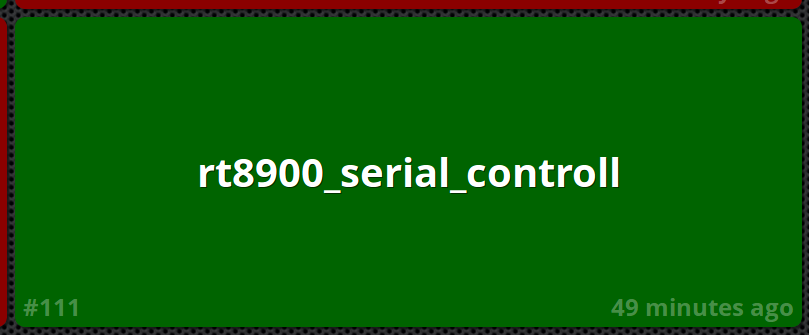
\includegraphics[width=0.5\textwidth]{img/CI_dashboard.png}
    \caption{A screenshot of the CI dashboard. This can be left open on a screen to track the build status. On failed builds this would turn red with a reason specified.}
    \label{fig:ci_dashboard}
\end{figure}

\begin{figure}
    \centering
    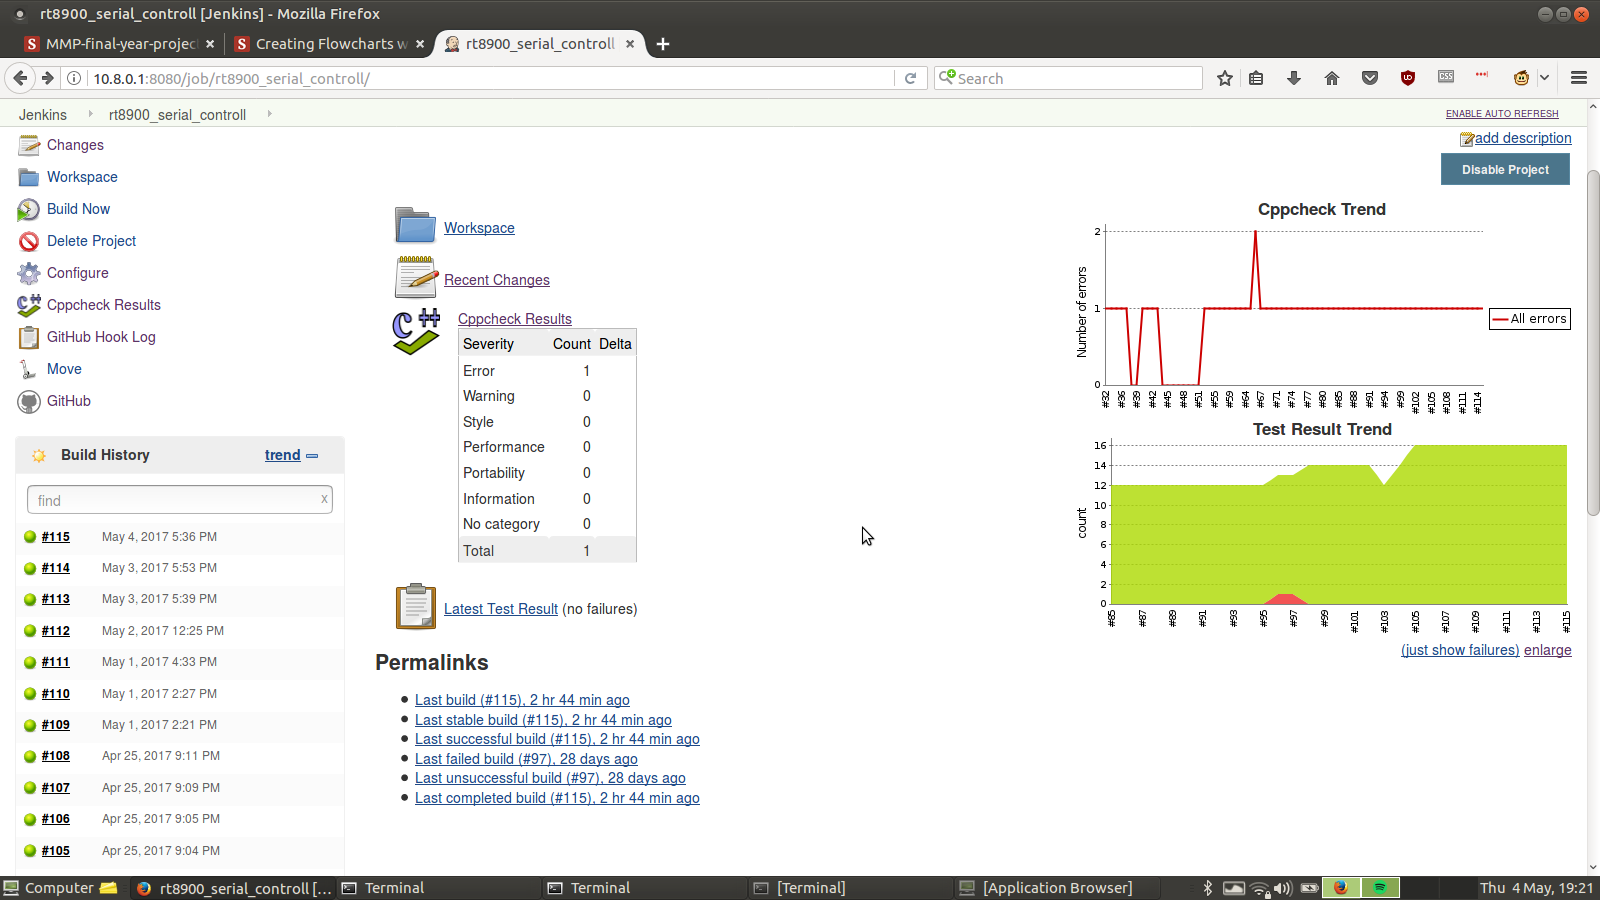
\includegraphics[width=1\textwidth]{img/jenkins_build.png}
    \caption[Jenkins build trends]{Jenkins showing test and error trends over time.}
    \label{fig:jenkins_build}
\end{figure}

\begin{figure}
    \centering
    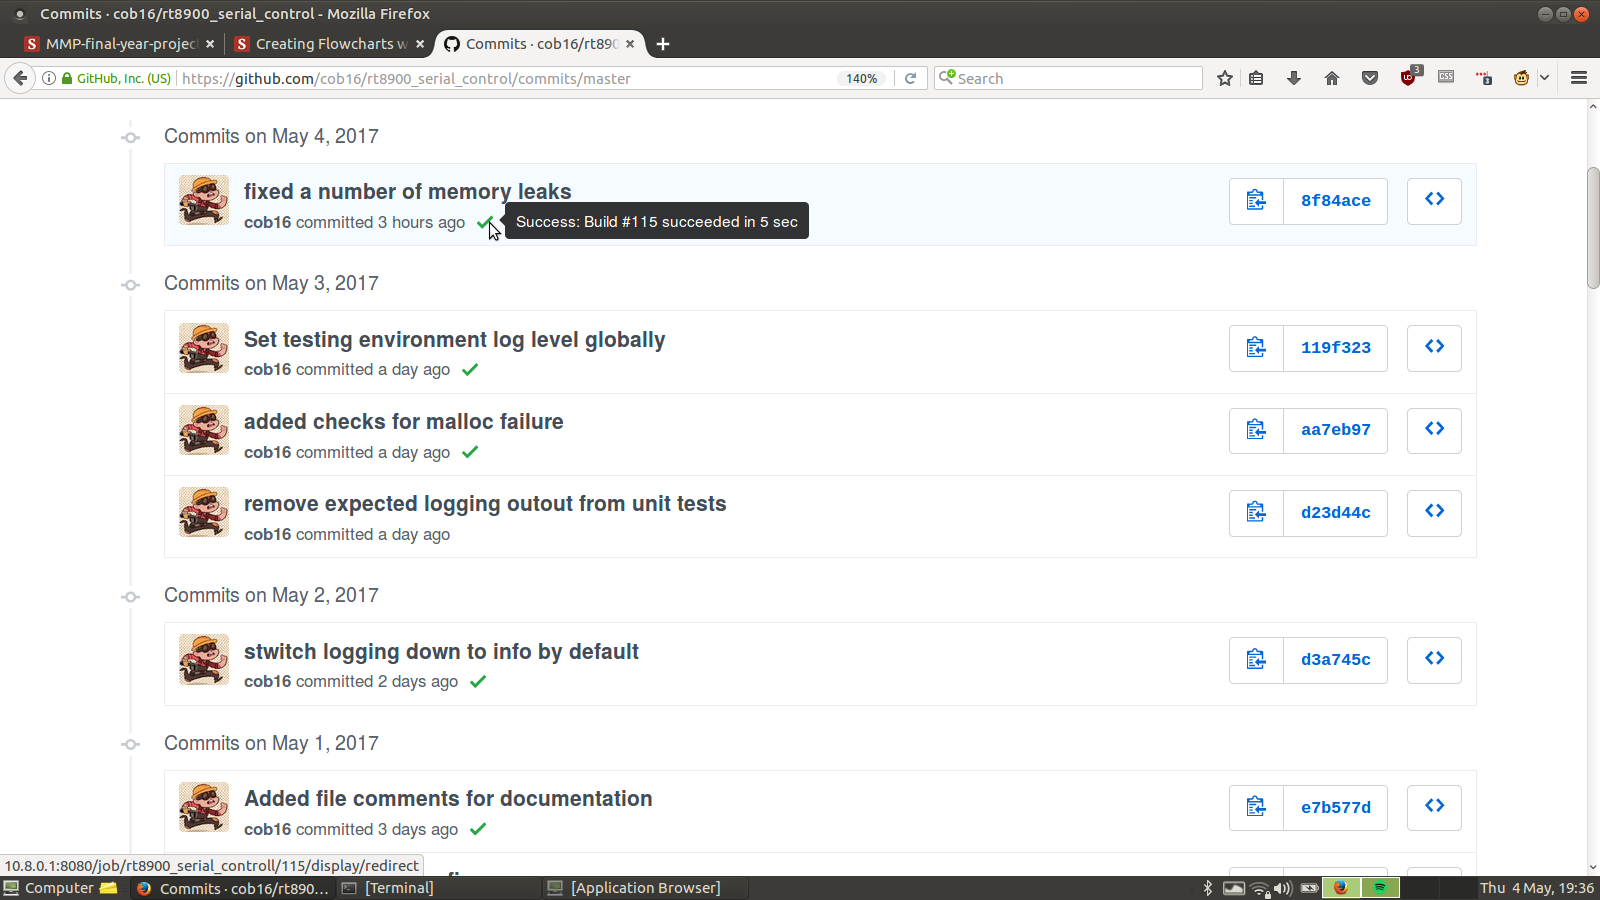
\includegraphics[width=1\textwidth]{img/github_commits.png}
    \caption[Tests on github]{Github commit list showing a tick on successful builds of each commit. This is useful historical information and is invaluable in preventing merges of unstable branches.}
    \label{fig:github_commits}
\end{figure}

\subsection{Unit Tests}
The project utilised unit tests throughout development (See appendix ~\ref{unit_test_output} for test output). This was an invaluable tool not only when refactoring but allowed development of the application outside of the lab where the radio was held while still being able to test the program.

\todo[]{talk about what functions were tested and how}

\section{Manual Testing}
Manual testing of the user shell was done by testing behaviour when expected and unexpected input was given. This was used to improve the user experience until a reasonably robust system had been made. User input is checked for the correct number of keywords and arguments. Arguments are safely cast to integers and range checked before being passed on to there corresponding functions. The input buffer dynamically reallocated up to a hard limit. The interrupt signal is handled appropriately so that the program can be shutdown at any time.

The application was also tested on a number of releases by watching a user with no prior experience with the system. Their feedback was accounted for by re-prioritising features as well as making tweaks to the interface to better meet users expectations. These test were combined by compiling and running the program on a separate system (see figure~\ref{fig:raspberry_pi})for that used during development to ensure that all necessary files were included in Git.

\begin{figure}[!h]
    \centering
    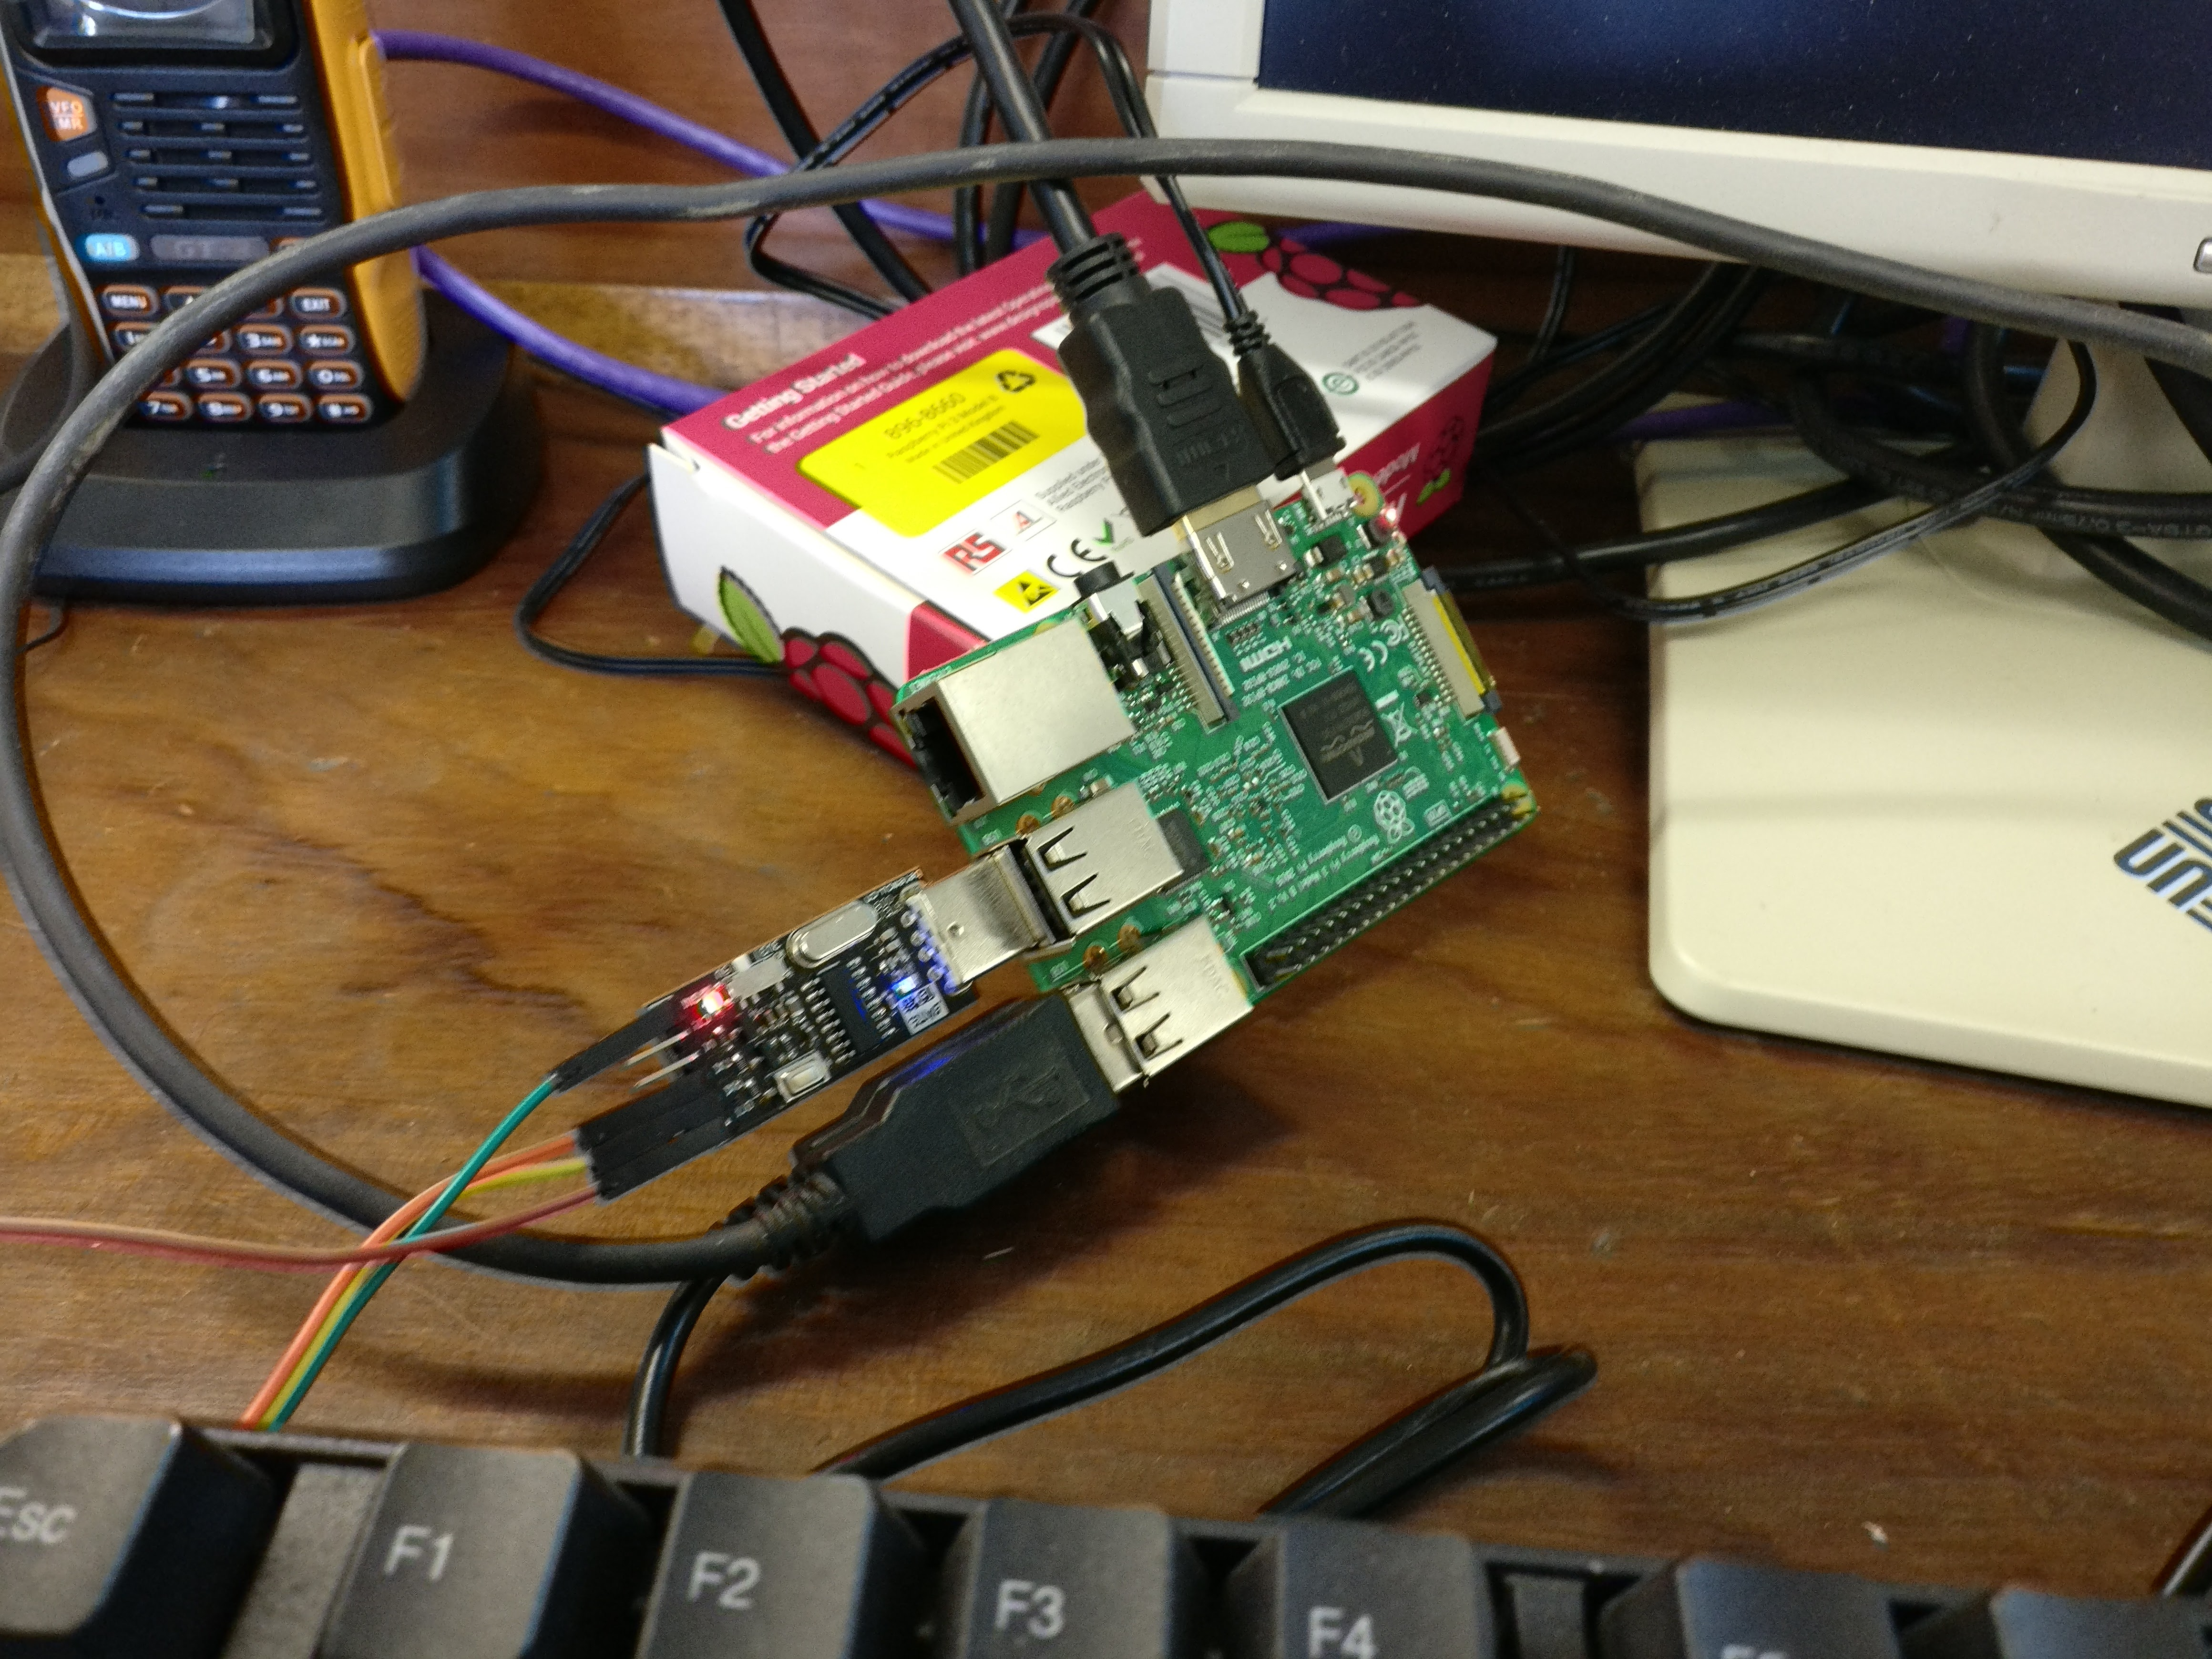
\includegraphics{img/raspberry_pi.jpg}
    \caption{A Raspberry Pi running the application}
    \label{fig:raspberry_pi}
\end{figure}

\todo[inline]{aceptance tests table}
Commands were checked to make sure their function worked as expected. This was done by cross-referencing the expected output with the output of the screen on the radio.

\subsection{Memory profiling}
Valgrind\cite{valgrind} was used to check for memory leaks in my program using this command.
\begin{minted}[breaklines]{bash}
valgrind --trace-children=yes --leak-check=full ./main/rt8900c -v5 /dev/ttyUSB0 
\end{minted}

This was an invaluable tool that found 4 leaks in the application. Its output also lists which function the memory was allocated to, making fixes easy. Massif was also used to measure the amount of memory that the application used (See figure~\ref{fig:memory_usage}). The peak memory usage of the application is 3.6 KiB. This peek occurs when a frequency is being dialled due to the large use of the sending queue to press each button in sequence. This is more than adequate for the current use-case, allowing for even the smallest microcontrollers to run the application.

\begin{minted}[breaklines]{bash}
valgrind --tool=massif ./rt8900_serial_control/cmake-build-debug/main/rt8900c -v5 /dev/ttyUSB0 
\end{minted}

\begin{figure}[H]
    \centering
    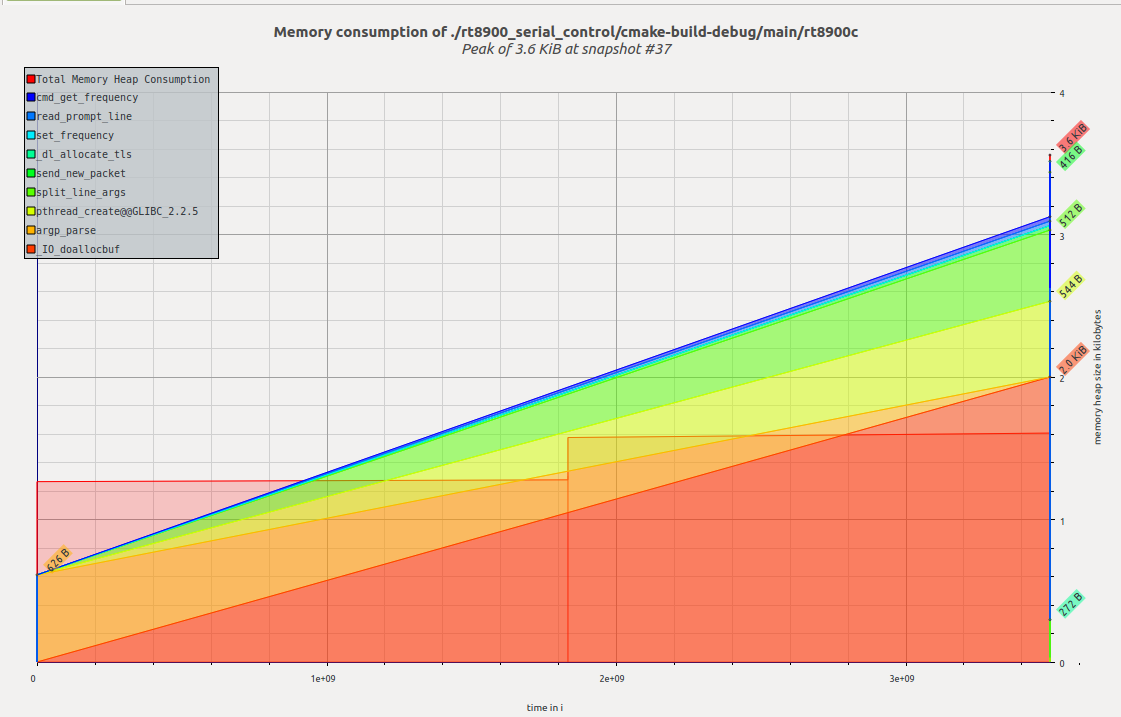
\includegraphics[width=1\textwidth]{img/memory_usage.png}
    \caption[Memory usage graph]{Memory usage of the application over time. This recording was done while the user tested every available function in the application.}
    \label{fig:memory_usage}
\end{figure}

\section{Known issues}
There were two known issues with the project at the time of submission. These issues were not deemed critical due to their current workarounds but are important improvements in development of the application.

\subsection*{Frequency validation}
Frequency validation follows the given list of frequencies from the user manual~\cite{user_manual}. However after testing, it was found that the right receiver supports only a subset of the frequencies that are listed. Further experimentation is required to discover this subset so that the validation can be correct for both receivers. This bug is limited in impact as upon receiving an invalid frequency the radio simply does nothing. In addition the user can see that the frequency was not changed from the output of the program.

\subsection*{Display packet reading}
\label{display_packet_reading}
Many functions that read and write packets currently have built in delays in order to give the radio time to send out a new display packet and to be processed by the reader thread. The true amount of time was not tested, therefore some functions sleep for as much as a second before continuing. This could be improved by implementing a get function that blocks until a new packet is received. The problem with this is that this provides a risk if a new packet is never received (as the function would then block forever). Ideally the program should try to recover by timing out and falling back to a last known safe packet. More research and analysis of solutions into reading the display packet would have helped to mitigate this.


\chapter{Evaluation}
% \begin{itemize}
%   \item Were the requirements correctly identified? 
%   \item Were the design decisions correct?
%   \item Could a more suitable set of tools have been chosen?
%   \item How well did the software meet the needs of those who were expecting to use it?
%   \item How well were any other project aims achieved?
%   \item If you were starting again, what would you do differently?
% \end{itemize}

\begin{figure}
\centering
\begin{verbatim}
------------------------------------------------------------------
Language      files          blank        comment           code
------------------------------------------------------------------
C                 7            233            174           1341
C/C++ Header     10            141            100            521
C++               4             68             43            246
CMake             4             22             15             60
------------------------------------------------------------------
SUM:             25            464            332           2168
------------------------------------------------------------------
\end{verbatim}
\caption[Project statistics]{The project source code at the time of submission contains 130 commits on 2168 lines of code primarily written in C.}
\label{fig:my_label}
\end{figure}

\section{Design Reflection}
The initial design of the application at the time was mostly adequate for the project. The structure of the program closely resembles what was planned in figure~\ref{overall_architecture}. It differs from the end result (See figure~\ref{fig:dependency_graph}) in the use of some utility files such as ``log.h'' and the standard lib includes. 

Greater research and design for the process of receiving and processing packets into the system could have been made. While the current system is adequate, its functions have to account for reading slightly delayed packets from the application buffer. This component of the system should be more efficient, as actions of the library will be expected to be as fast as possible, especially if the action is linked to a simple button in a GUI application.

\begin{figure}[h!]
    \centering
    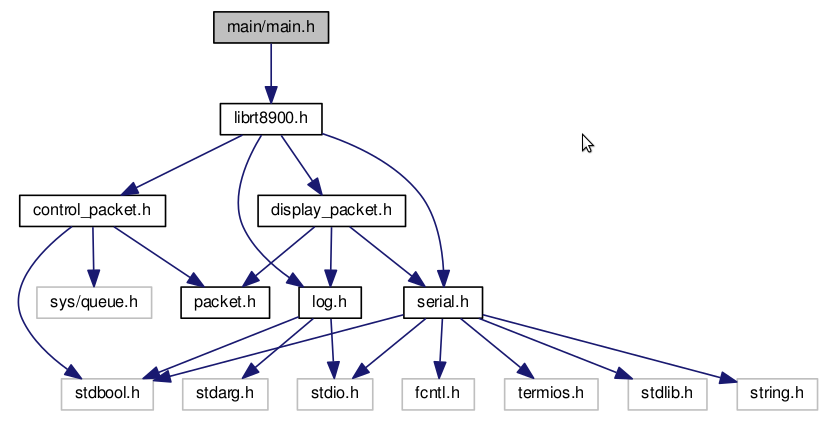
\includegraphics[width=1\textwidth]{img/dependancy_graph.png}
    \caption[Dependency graph]{Graph of the entire application dependency tree. This includes all standard library usages. The graph differs from the designed architecture in the use of a number of utility files such as serial.h and log.h}
    \label{fig:dependency_graph}
\end{figure}

\section{Suitability of tools}
\subsection*{C}
C was the best choice for this project in order to work as closely with data structures and serial interfaces. The relatively small size and low use of strings in the project contributed to the suitability of using the C language. Initially, unit tests with C++ prohibited certain C11 functions, however this was remedied with proper library linking. Compilation was exceedingly quick. Tools where always included directly in Linux distribution package managers unlike many other languages such as Python that use their own. 

\subsection*{Jenkins}
Using Jenkins over some of the free online platforms was a superior choice as it provided a better amount of customisation for the builds. For example, the build was able to use executables such as Cppcheck and GCC from the host system. Using a dedicated system over a service gave faster builds as well as more reliable time metrics so the build time could be monitored effectively.

\subsection*{Git}
Even for a single developer, the use of git helped maintain changes between computers. Fixes could occur in the lab while new features could be simultaneously developed on a separate branch for easy merges later. This helped fuel the ability to make quick changes without fear of versioning problems. The commit log helped to document changes, helping to review iterations for the blog posts as well as for this report. 

\section{Improvements}

After the second iteration, the length of iteration cycle could have been shortened from the two week period down to one. This was evident in the later iterations, as these contained many more features, therefore they could be shortened so that the iterations remained more focused. A reduction down to a single week iteration was mistakenly forgone for the sake of consistency of iteration lengths. 

The \gls{cli} was an expected feature, however it was an oversight to not provide an overall design for it. Stories and acceptance tests could have been made for these at the beginning of the project. This resulted in significant re-factoring in the last iteration in order to improve the overall code quality and maintainability of the shell. Better research and planning of a \gls{cli} as well as the the display packet reading thread earlier would have avoided difficulty in determining the testing latency later.

It was found out later that the targeted radio was the FT-8900r has a number of variants for each region. This is a problem as these models differ in their allowed frequencies for transmission. Currently only the Europe version is properly supported, with the US and Asia regions missing their configuration. This was a problem as it was difficult to source the frequency lists. In the future the likely solution would to have a number of lists for transmission that can be chosen via an optional flag to choose the model at runtime.

Unit tests were written primarily for library functions that manipulated packets. Testing of the actual user interface by capturing input and output of the program may have been a useful automation in order to decrease the time spent testing. During implementation this was not a priority due to how quick manual testing to the same end was. It can be foreseen however, that this would become more difficult in the future, as more and more features are added to the project.

The most useful development in the future would be to add an inter process communication method. The user shell would be moved out to a separate client that would talk to the server via a socket. This would allow other applications to utilise the socket \gls{8900} control such as Hamlib with a small patch. This would also permit making the \gls{cli} in another language, which may have facilitated faster development.

\section{Objectives}

\begin{table}[H]
\centering
\begin{tabular}{l|l}
Objective & Status \\
\hline
Final report & Complete \\
Frequency & Complete \\
Push to talk & Complete \\
Volume & Complete \\
Squelch & Complete \\
Power & Complete \\
Powering on the radio & Partial (Completed in software) \\
Code documentation & Complete \\
Schematic & Complete
\end{tabular}
\caption{List of objectives/deliverables}
\label{table:objectives}
\end{table}

It is the opinion of the developer that the project aims have been met. Users of the application have been provided with a useful, portable and fast application to control their \gls{8900} radios without the high cost of existing solutions. The hardware requirement of turning on the radio was only partially met. However a remote shack could still easily leave their radio on, ready for transmission (the radio will not consume much power when idle). For audio the data port at the back of the radio already provides this function. A good experience for a remote shack operator can be made with the use of a VOIP application such as Mumble~\cite{mumble} for audio and SSH to control the project application.
% add any additional chapters here

\setemptyheader

% \newacronym[longplural={Frames per Second}]{fpsLabel}{FPS}{Frame per Second}

\newacronym{cat}{CAT}{Computer Aided Transceiver}

\newacronym[]{8900}{FT-8900}{Yaesu FT-8900R}

\newacronym[]{tx}{TX}{serial transmission to the radio}
\newacronym[]{rx}{RX}{serial transmission from the radio}

\newacronym[]{ttl}{TTL}{Transistor to transistor logic}
\newacronym[]{dtr}{DTR}{Data Terminal Ready}

\newacronym[]{cli}{CLI}{command line interface}
\newacronym[]{api}{API}{application programming interface}

\newacronym[]{xp}{XP}{extreme programming}
\newacronym[]{fdd}{FDD}{feature driven development}

\newacronym[]{crc}{CRC}{Class, Responsibilities, and Collaboration}
\newacronym[]{rgf}{RGR}{Red, Green, Refactor}

\newacronym[]{ptt}{PTT}{push-to-talk}


\newglossaryentry{MOSFET}{
  name=MOSFET,
  description={MOSFET stands for metal–oxide–semiconductor field-effect transistor. This can be used as a digital switch that is opened and closed when a signal voltage is given to its gate pin.}
}

 \newglossaryentry{doxygen}
{
  name=Doxygen,
  description={A tool that generates documentation from source code}
}

\newglossaryentry{squelch}
{
  name=Squelch,
  description={Mutes the radio until a strong enough signal is detected. This has the effect of hiding background ``white noise'' when there is no incoming signal.}
}

\newglossaryentry{fuzzing}
{
  name=Fuzzing,
  description={Feeding random or unexpected data into a program in order to exploit or crash an application. A well known example is to cause a buffer overflow when trying to store the input in memory}
}


\printglossary

\addcontentsline{toc}{chapter}{Appendices}
\chapter*{Appendices}

\pagebreak

% start the appendix - sets up different numbering
\fancypagestyle{plain}{%
%\fancyhf{} % clear all header and footer fields
\fancyhead[L]{\textsl{Appendix\ \thechapter}}
\fancyhead[R]{\textsl{\leftmark}}}

\appendix
\fancyhead[L]{\textsl{Appendix\ \thechapter}}
\fancyhead[R]{\textsl{\leftmark}}
\fancyhead[C]{}
\fancyfoot[C]{\thepage}
\renewcommand{\headrulewidth}{0.4pt}
\renewcommand{\chaptermark}[1]{\markboth{#1}{}}

\fancyhead[L]{\textsl{Appendix\ \thechapter}}
\fancyhead[R]{\textsl{\leftmark}}
\fancyfoot[C]{{\thepage} of \pageref{LastPage}}

\chapter{Third-Party Code and Libraries}

\section*{Google Test}
The unit tests for this project where written in the Google test framework\cite{google_tests} without modification. This project is under the 2-Clause BSD Licenece and can be found at: \url{https://github.com/google/googletest /blob/master/googletest/LICENSE}.

\section*{Queue.h}
The <sys/queue.h> library is technically not part of the standard library (only de-facto). It was use to create a First in last out queue for the sender thread. This was used as it was available on targeted platforms therefore there was no requirement to re-implement. It is licenced under the 3-Clause BSD and can be found at \url{http://man7.org/linux/man-pages/man3/queue.3.license.html}.

\section*{Doxygen}
A documentation generator that parses source code to produce output in HTML or latex (among others). Licenced under the GPL v2. This can be found at \url{https://www.gnu.org/licenses/old-licenses/gpl-2.0.html}.


\chapter{Ethics Submission}
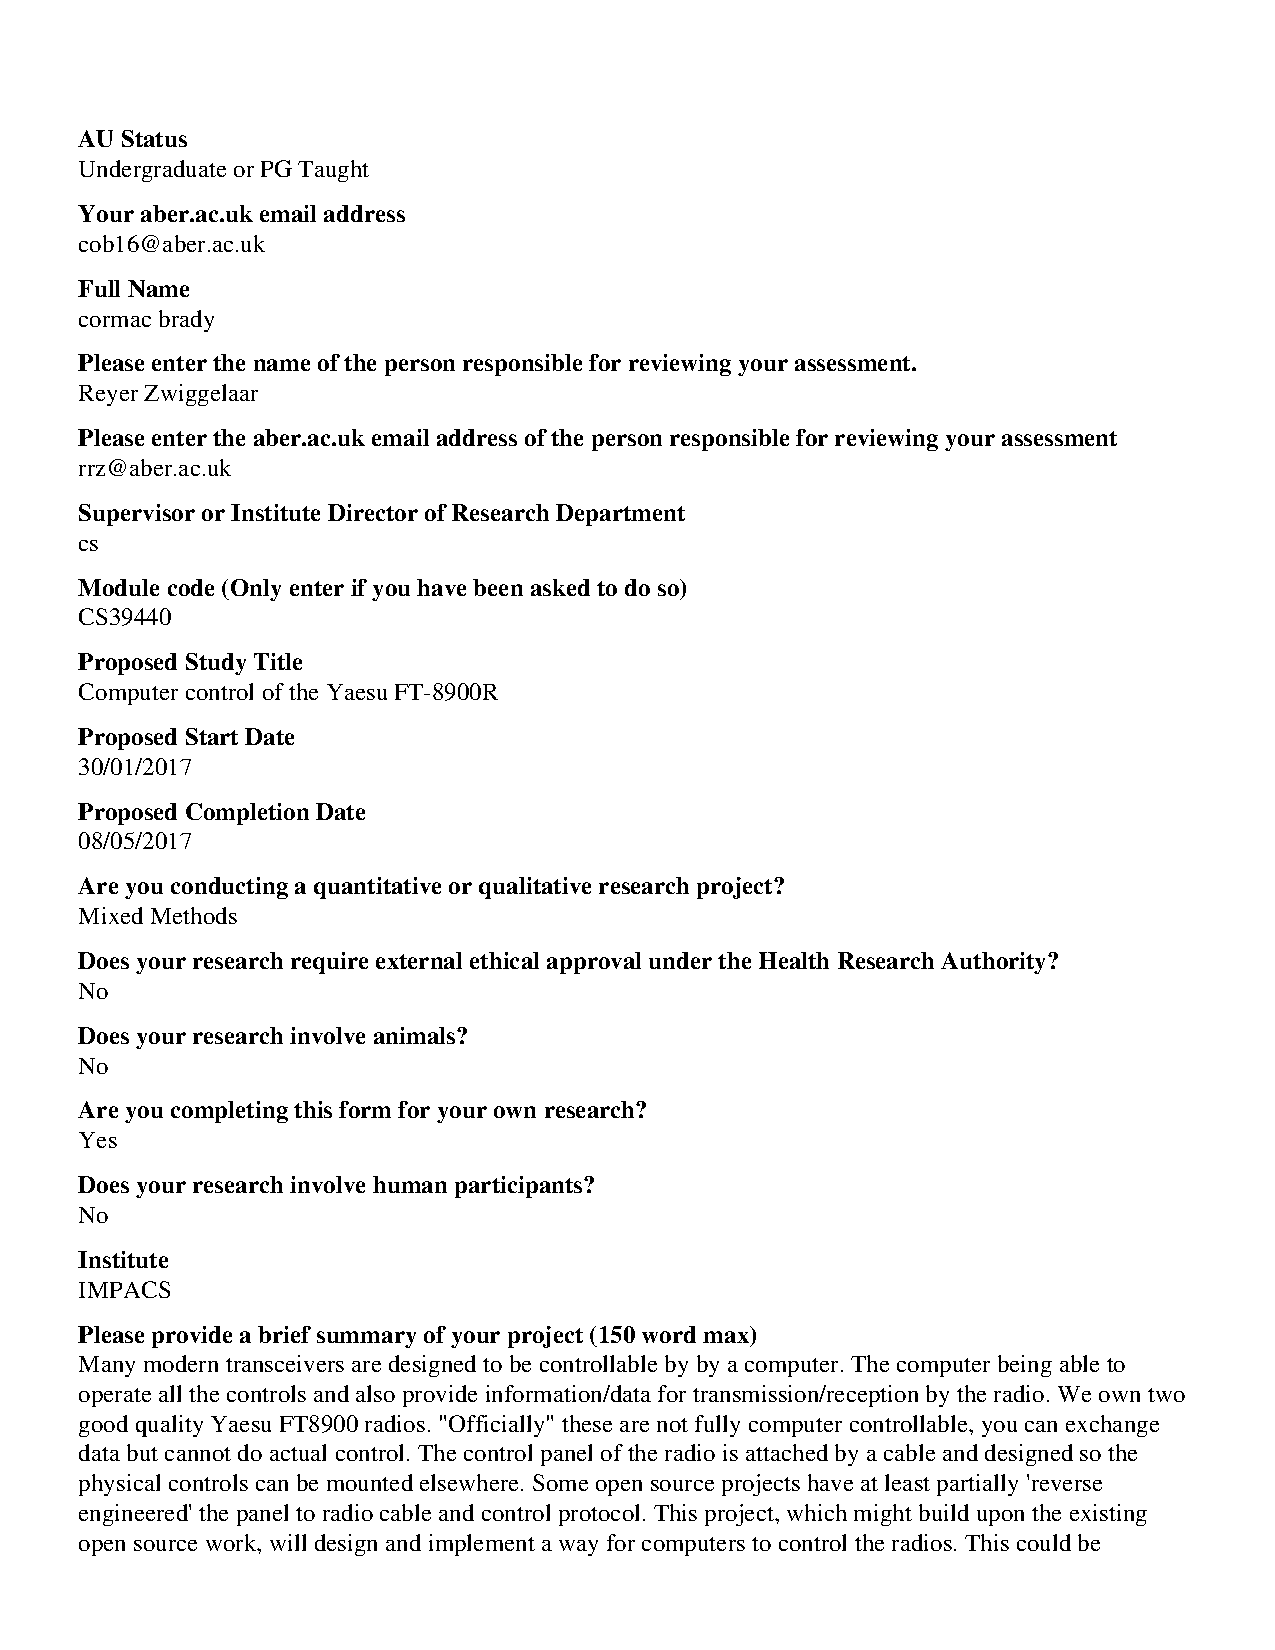
\includepdf[pages=-]{ethics_form.pdf}
\chapter{Code Examples}

\section{Python Bitfield}
\label{python_bitfield}
\begin{minted}[breaklines]{python}
from enum import Enum
import bits_mod

""""
would use 'pyserial' and bits_mod (or more useful rewrite)
This allows us to store the packet inside a long. 
Perhaps the most dense data structure for this problem.
"""


class EndBit(Enum):
    """This ENUM defines what the most significant bit should be. 
    The first byte should end with 1 else 0"""
    FIRST_BYTE = 1
    OTHER_BYTE = 0


class PacketByte:
    """This class allows easy manipulation, conversion and handling of our 
    packet bytes"""

    def __init__(self, data_bytes, endbit):
        if endbit in EndBit:
            self._endbit = endbit

         # this will through ValueError back if it fails
        self.data_bytes = int(data_bytes, 2)  


packet = bits_mod.Bits(104)


def packet_range(start, stop):
    """Range wrapper that auto works in reverse"""
    if start <= stop:
        return list(range(start, stop))
    else:
        return list(range(start, stop, -1))


#how map coule be represented
packet_map = {
    'left_encoder': packet_range(0, 7),
    'right_encoder': packet_range(8, 15),
    'well_made_function': [2, 44, 45] + packet_range(90, 104),
}

for i in packet_map['left_encoder']:
    if i % 2 != 0:
        packet.mark(i)


def get_bits(array_of_indexes):
    bits = b''
    for i in array_of_indexes:
        if packet.is_true(i):
            bits += b'1'
        else:
            bits += b'0'
    return bits


print(get_bits(packet_map['left_encoder'])) #get related bytes


def test_mapping_ranges(packet_map):
    expected_range = set(range(0, 104))
    actual_range = set()
    for i in packet_map.values():
        
        # see if there are overlapping mappings
        if actual_range.intersection() is None: 
            actual_range.add(i)
        else:
            pass #fail out as there are overlapping maps
    if set(range(0, 104)).difference(actual_range) is not None:
pass # fail as there are missing mappings
\end{minted}


\section{Unit test output}
\label{unit_test_output}
\begin{verbatim}
[==========] Running 16 tests from 6 test cases.
[----------] Global test environment set-up.
[----------] 4 tests from TestDisplayPacket
[ RUN      ] TestDisplayPacket.test_find_packet_start
[       OK ] TestDisplayPacket.test_find_packet_start (0 ms)
[ RUN      ] TestDisplayPacket.test_shift_array
[       OK ] TestDisplayPacket.test_shift_array (0 ms)
[ RUN      ] TestDisplayPacket.test_get_range
[       OK ] TestDisplayPacket.test_get_range (0 ms)
[ RUN      ] TestDisplayPacket.test_operational_range
[       OK ] TestDisplayPacket.test_operational_range (0 ms)
[----------] 4 tests from TestDisplayPacket (0 ms total)

[----------] 3 tests from TestDisplayPacketReaders
[ RUN      ] TestDisplayPacketReaders.test_read_busy
[       OK ] TestDisplayPacketReaders.test_read_busy (0 ms)
[ RUN      ] TestDisplayPacketReaders.test_packet_read
[       OK ] TestDisplayPacketReaders.test_packet_read (0 ms)
[ RUN      ] TestDisplayPacketReaders.test_read_14_seg
[       OK ] TestDisplayPacketReaders.test_read_14_seg (0 ms)
[----------] 3 tests from TestDisplayPacketReaders (0 ms total)

[----------] 2 tests from Librt8900Test
[ RUN      ] Librt8900Test.test_in_freq_range
[       OK ] Librt8900Test.test_in_freq_range (0 ms)
[ RUN      ] Librt8900Test.test_current_freq_valid
[       OK ] Librt8900Test.test_current_freq_valid (0 ms)
[----------] 2 tests from Librt8900Test (0 ms total)

[----------] 2 tests from ControlPacketTest
[ RUN      ] ControlPacketTest.PACKET_BYTE
[       OK ] ControlPacketTest.PACKET_BYTE (0 ms)
[ RUN      ] ControlPacketTest.CONTROL_PACKET
[       OK ] ControlPacketTest.CONTROL_PACKET (0 ms)
[----------] 2 tests from ControlPacketTest (1 ms total)

[----------] 2 tests from TestKeypadButtons
[ RUN      ] TestKeypadButtons.test_set_button
[       OK ] TestKeypadButtons.test_set_button (0 ms)
[ RUN      ] TestKeypadButtons.test_button_from_int
[       OK ] TestKeypadButtons.test_button_from_int (0 ms)
[----------] 2 tests from TestKeypadButtons (0 ms total)

[----------] 3 tests from TestAPISetters
[ RUN      ] TestAPISetters.test_safe_int_char
[       OK ] TestAPISetters.test_safe_int_char (0 ms)
[ RUN      ] TestAPISetters.test_set_L_R_volume
[       OK ] TestAPISetters.test_set_L_R_volume (0 ms)
[ RUN      ] TestAPISetters.test_set_L_R_squelch
[       OK ] TestAPISetters.test_set_L_R_squelch (0 ms)
[----------] 3 tests from TestAPISetters (0 ms total)

[----------] Global test environment tear-down
[==========] 16 tests from 6 test cases ran. (1 ms total)
[  PASSED  ] 16 tests.
\end{verbatim}
\chapter{Code Documentation}
This contains a copy of the auto generated code documentation. Some sections are very useful to consult, however this print version is less so than the HTML version. The HTML version can attained ether by flowing the README.md instructions or by navigating to:

\url{https://cormacbrady.info/rt8900_docs/}

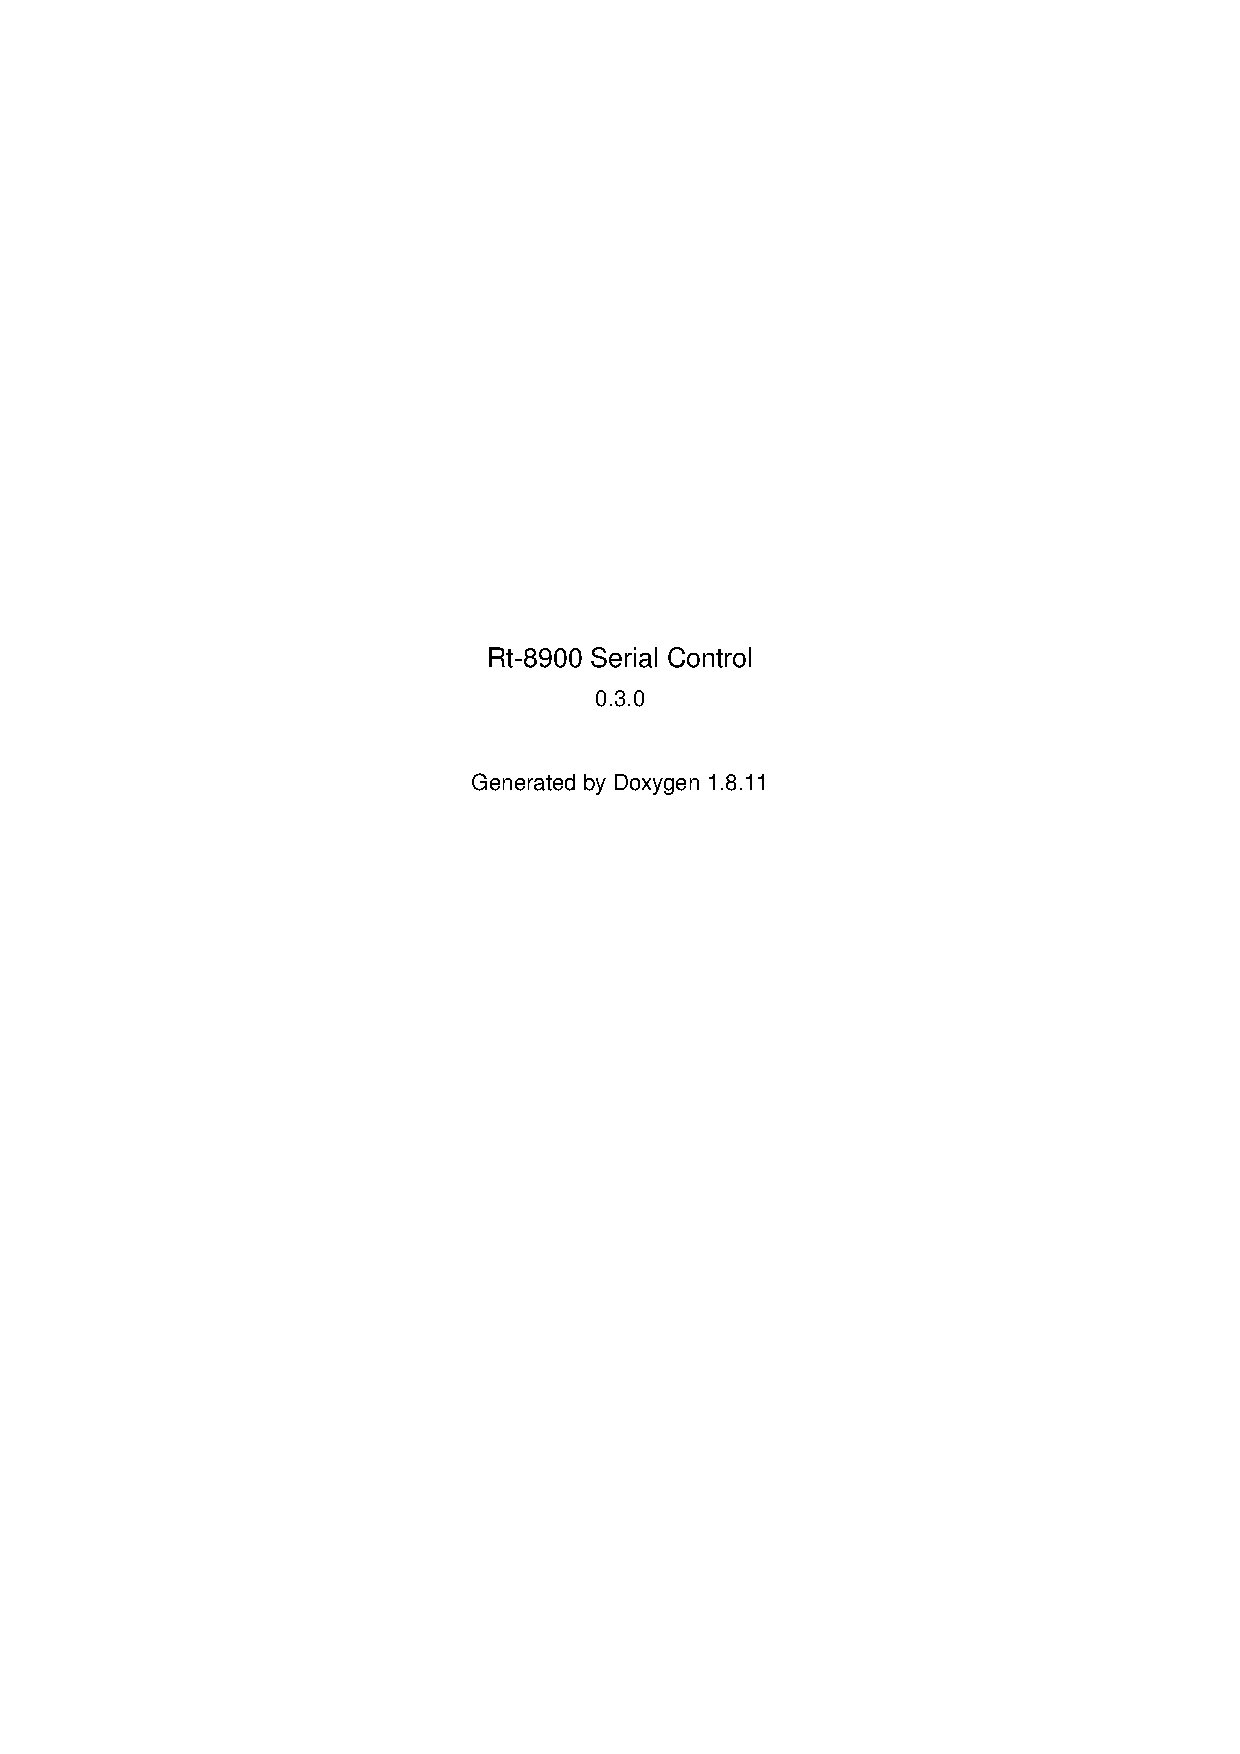
\includepdf[pages=-]{code-doc.pdf}


\fancypagestyle{plain}{%
   \fancyhead{} %[C]{Annotated Bibliography}
   \fancyfoot[C]{{\thepage} of \pageref{LastPage}} % except the center
   \renewcommand{\headrulewidth}{0pt}
   \renewcommand{\footrulewidth}{0pt}
}

\setemptyheader

\nocite{*} % include everything from the bibliography, irrespective of whether it has been referenced.

% the following line is included so that the bibliography is also shown in the table of contents. There is the possibility that this is added to the previous page for the bibliography. To address this, a newline is added so that it appears on the first page for the bibliography. 
\addcontentsline{toc}{chapter}{Annotated Bibliography} % Adds References to contents page

%
% example of including an annotated bibliography. The current style is an author date one. If you want to change, comment out the line and uncomment the subsequent line. You should also modify the packages included at the top (see the notes earlier in the file) and then trash your aux files and re-run. 
%\bibliographystyle{authordate2annot}
\bibliographystyle{IEEEannotU}
\renewcommand{\bibname}{Annotated Bibliography} 

\bibliography{99-references} % References file

\end{document}
